\documentclass{sigplanconf}

\usepackage{lgrind}
\usepackage[dvips]{graphicx}
\usepackage{verbatim}
\pagestyle{plain}

%% This bit allows you to either specify only the files which you wish to
%% process, or `all' to process all files which you \include.
%% Krishna Sethuraman (1990).

\typein [\files]{Enter file names to process, (chap1,chap2 ...), or `all' to
process all files:}
\def\all{all}
\ifx\files\all \typeout{Including all files.} \else \typeout{Including only \files.} \includeonly{\files} \fi

\begin{document}

% -*-latex-*-
% $Log: not supported by cvs2svn $
% Revision 1.7  2001/02/08 18:53:16  boojum
% changed some \newpages to \cleardoublepages
%
% Revision 1.6  1999/10/21 14:49:31  boojum
% changed comment referring to documentstyle
%
% Revision 1.5  1999/10/21 14:39:04  boojum
% *** empty log message ***
%
% Revision 1.4  1997/04/18  17:54:10  othomas
% added page numbers on abstract and cover, and made 1 abstract
% page the default rather than 2.  (anne hunter tells me this
% is the new institute standard.)
%
% Revision 1.4  1997/04/18  17:54:10  othomas
% added page numbers on abstract and cover, and made 1 abstract
% page the default rather than 2.  (anne hunter tells me this
% is the new institute standard.)
%
% Revision 1.3  93/05/17  17:06:29  starflt
% Added acknowledgements section (suggested by tompalka)
%
% Revision 1.2  92/04/22  13:13:13  epeisach
% Fixes for 1991 course 6 requirements
% Phrase "and to grant others the right to do so" has been added to
% permission clause
% Second copy of abstract is not counted as separate pages so numbering works
% out
%
% Revision 1.1  92/04/22  13:08:20  epeisach
\title{Language and Compiler Support for Stream Programs}

\author{William Thies}
\department{Department of Electrical Engineering and Computer Science}
% If the thesis is for two degrees simultaneously, list them both
% separated by \and like this:
% \degree{Doctor of Philosophy \and Master of Science}
%\degree{Doctor of Philosophy of Science in Computer Science and Engineering}
\degree{Doctor of Philosophy}
\degreemonth{September} \degreeyear{2008} \thesisdate{\today}

\prevdegrees{~ \\ 
Bachelor of Science, Computer Science and Engineering\\
Massachusetts Institute of Technology, 2001 \\
~ \\
Bachelor of Science, Mathematics\\
Massachusetts Institute of Technology, 2002 \\
~ \\
Master of Engineering, Computer Science and Engineering \\
Massachusetts Institute of Technology, 2002 \\
~ \\
}

%% By default, the thesis will be copyrighted to MIT.  If you need to copyright
%% the thesis to yourself, just specify the `vi' documentclass option.  If for
%% some reason you want to exactly specify the copyright notice text, you can
%% use the \copyrightnoticetext command.
%\copyrightnoticetext{\copyright IBM, 1990.  Do not open till Xmas.}

% If there is more than one supervisor, use the \supervisor command
% once for each.
\supervisor{Saman Amarasinghe}{Associate Professor}

% These are optional, and enabled with reader.sty
%\reader{Arvind}{Professor}
%\reader{Srini Devadas}{Professor}

% This is the department committee chairman, not the thesis committee
% chairman.  You should replace this with your Department's Committee
% Chairman.
\chairman{Terry P. Orlando}{Chair, Department Committee on Graduate Students}

% Make the titlepage based on the above information.  If you need
% something special and can't use the standard form, you can specify
% the exact text of the titlepage yourself.  Put it in a titlepage
% environment and leave blank lines where you want vertical space.
% The spaces will be adjusted to fill the entire page.  The dotted
% lines for the signatures are made with the \signature command.
\maketitle

% The abstractpage environment sets up everything on the page except
% the text itself.  The title and other header material are put at the
% top of the page, and the supervisors are listed at the bottom.  A
% new page is begun both before and after.  Of course, an abstract may
% be more than one page itself.  If you need more control over the
% format of the page, you can use the abstract environment, which puts
% the word "Abstract" at the beginning and single spaces its text.

%% You can either \input (*not* \include) your abstract file, or you can put
%% the text of the abstract directly between the \begin{abstractpage} and
%% \end{abstractpage} commands.

% First copy: start a new page, and save the page number.
\cleardoublepage
% Uncomment the next line if you do NOT want a page number on your
% abstract and acknowledgments pages.
% \pagestyle{empty}
\setcounter{savepage}{\thepage}
\begin{abstractpage}
As DSP programming is becoming more complex, there is an increasing
need for high-level abstractions that can be efficiently compiled.
Toward this end, we present a set of aggressive optimizations that
target linear sections of a stream program.  Our input language is
StreamIt, which represents programs as a hierarchical graph of
autonomous filters.  A filter is linear if each of its outputs can be
represented as an affine combination of its inputs.  Linear filters
are common in DSP applications; examples include FIR filters,
expanders, compressors, FFTs and DCTs.

We present a linear extraction analysis that automatically detects
linear filters based on the C-like code in their {\tt work} function.
Once linear filters are identified, we show how neighboring nodes can
be collapsed into a single linear representation, thereby eliminating
many redundant computations.  Also, we describe a method for
automatically translating linear nodes into the frequency domain,
thereby yielding algorithmic savings for convolutional filters.

We have completed a fully-automatic implementation of the above
techniques as part of the StreamIt compiler, and we demonstrate
performance improvements that average 400\% over our benchmark
applications.




\end{abstractpage}

% Additional copy: start a new page, and reset the page number.  This way,
% the second copy of the abstract is not counted as separate pages.
% Uncomment the next 6 lines if you need two copies of the abstract
% page.
% \setcounter{page}{\thesavepage}
% \begin{abstractpage}
% As DSP programming is becoming more complex, there is an increasing
need for high-level abstractions that can be efficiently compiled.
Toward this end, we present a set of aggressive optimizations that
target linear sections of a stream program.  Our input language is
StreamIt, which represents programs as a hierarchical graph of
autonomous filters.  A filter is linear if each of its outputs can be
represented as an affine combination of its inputs.  Linear filters
are common in DSP applications; examples include FIR filters,
expanders, compressors, FFTs and DCTs.

We present a linear extraction analysis that automatically detects
linear filters based on the C-like code in their {\tt work} function.
Once linear filters are identified, we show how neighboring nodes can
be collapsed into a single linear representation, thereby eliminating
many redundant computations.  Also, we describe a method for
automatically translating linear nodes into the frequency domain,
thereby yielding algorithmic savings for convolutional filters.

We have completed a fully-automatic implementation of the above
techniques as part of the StreamIt compiler, and we demonstrate
performance improvements that average 400\% over our benchmark
applications.




% \end{abstractpage}

\cleardoublepage

\newpage
~ \vspace{-3.7\baselineskip}\\
\enlargethispage{0.3\baselineskip}
\section*{Acknowledgments}

I would like to start by expressing my deepest gratitude to my
advisor, colleague and friend, Saman Amarasinghe.
%Saman's committment to me has been downright scary.
%Simply put, Saman has changed my life.
%Simply put, Saman has been the mentor of a lifetime.
From 4am phone calls in Boston to weeks of one-on-one time in Sri
Lanka and India, Saman invested {\it unfathomable} time and energy
into my development as a researcher and as a person.  His extreme
creativity, energy, and optimism (not to mention mad PowerPoint
skills!) have been a constant source of inspiration, and whenever I am
at my best, it is usually because I am asking myself: {\it What would
Saman do}?  Saman offered unprecedented freedom for me to pursue
diverse interests in graduate school -- including weeks at a time
working with other groups -- and served as a fierce champion on my
behalf in every possible way.  I will forever treasure our deep sense
of shared purpose and can only aspire to impact others as much as he
has impacted me.

%Like a Papa Bear, any arguments between the two of us would be 
%completely dwarfed by the fierce battles he would wage on my behalf.

\vspace{-8pt}\paragraph*{Contributors to this dissertation} Many
people made direct contributions to the content of this dissertation.
The StreamIt project was a fundamentally collaborative undertaking,
involving the extended efforts of over 27 people.  I feel very lucky
to have been part of such an insightful, dedicated, and fun team.
Section~\ref{sec:streamit-project} provides a technical overview of
the entire project, including the division of labor.  In what follows
I am listing only a subset of each person's actual contributions.
Michael Gordon, my kindred Ph.D. student throughout the entire
StreamIt project, led the development of the parallelization
algorithms (summarized in Chapter~4), the Raw backend and countless
other aspects of the compiler.  Rodric Rabbah championed the project
in many capacities, including contributions to cache optimizations
(summarized in Chapter~4), teleport messaging (Chapter~3), the MPEG2
benchmarks, an Eclipse interface, and the Cell backend.  Michal
Karczmarek was instrumental in the original language design (Chapter
2) and teleport messaging, and also implemented the StreamIt scheduler
and runtime library.  David Maze, Jasper Lin, and Allyn Dimock made
sweeping contributions to the compiler infrastructure; I will forever
admire their skills and tenacity in making everything work.

Central to the StreamIt project is an exceptional array of
M.Eng. students, who I feel very privileged to have interacted with
over the years.  Andrew Lamb, Sitij Agrawal, and Janis Sermulins led
the respective development of linear optimizations, linear statespace
optimizations, and cache optimizations (all summarized in Chapter~4).
Janis also implemented the cluster backend, with support for teleport
messaging (providing results for Chapter~3).  Matthew Drake
implemented the MPEG2 codec in StreamIt, while Jiawen Chen implemented
a flexible graphics pipeline and Basier Aziz implemented mosaic
imaging.  Daviz Zhang developed a lightweight streaming layer for the
Cell processor; Kimberly Kuo developed an Eclipse user interface for
StreamIt; Juan Reyes developed a graphical editor for stream graphs;
and Jeremy Wong modeled the scalability of stream programs.  Kunal
Agrawal investigated bit-level optimizations in StreamIt.  Ceryen Tan
is improving StreamIt's multicore backend.

The StreamIt project also benefited from an outstanding set of
undergraduate researchers, who taught me many things.  Ali Meli, Chris
Leger, Satish Ramaswamy, Matt Brown, and Shirley Fung made important
contributions to the StreamIt benchmark suite (detailed in Chapter~2).
Steve Hall integrated compressed-domain transformations into the
StreamIt compiler (providing results for Chapter~5).  Qiuyuan Li
worked on a StreamIt backends for Cell, while Phil Sung targeted a
GPU.

%Qiuyuan Li worked on a StreamIt backend for the Cell processor, while
%Phil Sung worked on a backend for graphics processors.

Individuals from other research groups also impacted the StreamIt
project.  Members of the Raw group offered incredible support for our
experiments, including Anant Agarwal, Michael Taylor, Walter Lee,
Jason Miller, Ian Bratt, Jonathan Eastep, David Wentzlaff, Ben
Greenwald, Hank Hoffmann, Paul Johnson, Jason Kim, Jim Psota, Nathan
Schnidman, and Matthew Frank.
%
\newpage
\enlargethispage{0.3\baselineskip}
%
~ \vspace{-1.3\baselineskip}\\
\noindent Hank Hoffmann, Nathan Schnidman, and Stephanie Seneff also
provided valuable expertise on designing and parallelizing signal
processing applications.  External contributors to the StreamIt
benchmark suite include Ola Johnsson, Mani Narayanan, Magnus
Stenemo, Jinwoo Suh, Zain ul-Abdin, and Amy Williams.  Fabrice
Rastello offered key insights for improving our cache optimizations.
Weng-Fai Wong offered guidance on several projects during his visit
to the group.  StreamIt also benefited immensely from regular and
insightful conversations with stakeholders from industry, including
Peter Mattson, Richard Lethin, John Chapin, Vanu Bose, and Andy Ong.

Outside of the StreamIt project, additional individuals made direct
contributions to this dissertation.  In developing our tool for
extracting stream parallelism (Chapter~6), I am indebted to Vikram
Chandrasekhar for months of tenacious hacking and to Stephen McCamant
for help with Valgrind.  I thank Jason Ansel, Chen Ding, Ronny
Krashinsky, Viktor Kuncak, and Alex Salcianu, who provided valuable
feedback on manuscripts that were incorporated into this dissertation.
I am also grateful to Arvind and Srini Devadas for serving on my
committee on very short notice, and to Marek Olszewski for serving as
my remote agent of thesis submission!

\vspace{-8pt}\paragraph*{The rest of the story} Throughout my life,
I have been extremely fortunate to have had an amazing set of
mentors who invested a lot of themselves in my personal growth.  I
thank Thomas ``Doc'' Arnold for taking an interest in a nerdy high
school kid, and for setting him loose with chemistry equipment in a
Norwegian glacier valley -- a tactic which cemented my interest in
science, especially the kind you can do while remaining dry.
%a tactic which ignited not only my interest in science, but also in
%girls.
I thank Scott Camazine for taking a chance on a high school programmer
in my first taste of academic research, an enriching experience which
%was not only enriching and fun, but also 
opened up many doors for me in the future.  I thank Vanessa Colella
and Mitchel Resnick for making my first UROP experience a very
special one, as evidenced by my subsequent addiction to the UROP
program.  I thank Andrew Begel for teaching me many things, not
least of which is by demonstration of his staggering commitment,
capacity, and all-around coolness in mentoring undergraduates.  I'm
especially grateful to Brian Silverman, a mentor and valued friend
whose unique perspectives on everything from Life in StarLogo to
life on Mars have impacted me more than he might know.  I thank
Markus Zahn for excellent advice and guidance, both as my
undergraduate advisor and UROP supervisor.  Finally, I'm very
grateful to Kath Knobe, who provided unparalleled mentorship during
my summers at Compaq and stimulated my first interest in compilers
research.

Graduate school brought a new set of mentors.  I learned a great
deal from authoring papers or proposals with Anant Agarwal, Srini
Devadas, Fredo Durand, Michael Ernst, Todd Thorsen, and
Fr\'{e}d\'{e}ric Vivien, each of whom exemplifies the role of a
faculty member in nurturing student talent.  I am also very grateful
to Srini Devadas, Martin Rinard, Michael Ernst, and Arvind for being
especially accessible as counselors, showing interest in my work and
well-being even in spite of very busy schedules.  I could not have
imagined a more supportive environment for graduate study.

I thank Charles Leiserson and Piotr Indyk for teaching me about
teaching itself.  I will always remember riding the T with Charles
when a car full of Red Sox fans asked him what he does for a living.
Imagining the impressive spectrum of possible replies, I should not
have been surprised when Charles said simply, ``I teach''.  Nothing
could be more true, and I feel very privileged to have been a TA in
his class.

I'd like to thank my collaborators on projects other than StreamIt,
for enabling fulfilling and fun pursuits outside 
% the work described in 
of this dissertation.  In the microfluidics lab, I thank
J.P. Urbanski for many late nights ``chilling at the lab'', his
euphemism for a recurring process whereby he manufactures chips and
I destroy them.  His knowledge, determination, and overall good
nature are truly inspiring.  I also learned a great deal from David
Craig, Mats Cooper, Todd Thorsen, and Jeremy Gunawardena, 
%
\newpage
\enlargethispage{0.5\baselineskip}
%
~ \vspace{-1.5\baselineskip}\\
\noindent who were extremely supportive of our foray into
microfluidics.  I thank Nada Amin for her insights, skills, and
drive in developing our CAD tool, and for being an absolute pleasure
to work with.

%In the microfluidics lab, I learned an immense amount from
%J.P. Urbanski, microfluidic wizard extraordinaire whose work ethic
%is as intense as it is understated -- never again will I think
%lightly of a late night ``chilling at the lab''.

I'm very thankful to my collaborators in applying technology towards
problems in socio-economic development, from whom I've drawn much
support.  First and foremost is Manish Bhardwaj, whose rare
combination of brilliance, determination, and selflessness has been
a deep inspiration to me.  I also thank Emma Brunskill, who has been
a tremendous collaborator on many fronts, as well as
%whose independence and resourcefulness are always humbling.  
%I'm very grateful to Emma Brunskill, Somani Patnaik, 
Sara Cinnamon, Goutam Reddy, Somani Patnaik and Pallavi Kaushik for
being incredibly talented, dedicated, and fun teammates.
%I thank the Venerable Tenzin Priyadarshi and Scott Kennedy for
%valuable support and guidance.
%
%Further in the past, 
I am very grateful to Libby Levison for involving me in my first
project at the intersection of technology and development, without
which I might have gone down a very different path.  I also thank
Samidh Chakrabarti for being a great officemate and friend, and my
first peer with whom I could investigate this space together.

I am indebted to the many students and staff who worked with me on
the TEK project, including Marjorie Cheng, Tazeen Mahtab, Genevieve
Cuevas, Damon Berry, Saad Shakhshir, Janelle Prevost, Hongfei Tian,
Mark Halsey, and Libby Levison.  I also thank Pratik Kotkar,
Jonathan Birnbaum, and Matt Aasted for their work on the Audio Wiki.
I would not have been able to accomplish nearly as much without the
%continuous 
insights, dedication, and hard work of all these individuals.

% leaving out sri lanka guys, since it's not released:
% - Thayaparan Kailainathan
% - Mahendrakumar Senthivel
% - Thayarupan Rajendram
%
% leaving out some TEK authors who I don't even know:
% - Alexandro Artola
% - Binh D. Vo
% - Yuliya Litvak
% - Sheldon Chan
% - Sid Henderson

Graduate school would be nothing if not for paper deadlines, and I
feel very lucky to have been down in the trenches with such bright,
dependable, and entertaining co-authors.  Of people not already cited
as such, I thank Marten van Dijk, Blaise Gassend, Andrew Lee, Charles
W. O'Donnell, Kari Pulli, Christopher Rhodes, Jeffrey Sheldon, David
Wentzlaff, Amy Williams, and Matthias Zwicker for some of the best
end-to-end research experiences I could imagine.

Many people made the office a very special place to be.  Mary McDavitt
is an amazing force for good, serving as my rock and foundation
throughout many administrative hurricanes; I can't thank her enough
for all of her help, advice, and good cheer over the years.  I'm also
very grateful to Shireen Yadollahpour, Cornelia Colyer, and Jennifer
Tucker, whose helpfulness I will never forget.  Special thanks to
Michael Vezza, system administrator extraordinaire, for his extreme
patience and helpfulness in tending to my every question, and fixing
everything that I broke.

I thank all the talented members of the Commit group, and especially
the Ph.D. students and staff -- Jason Ansel, Derek Bruening, Vikram
Chandrasekhar, Gleb Chuvpilo, Allyn Dimock, Michael Gordon, David
Maze, Michal Karczmarek, Sam Larsen, Marek Olszewski, Diego Puppin,
Rodric Rabbah, Mark Stephenson, Jean Yang, and Qin Zhao.  On top of
tolerating {\it way} more than their fair share of StreamIt talks,
they offered the best meeting, eating, and traveling company ever.  I
especially thank Michael Gordon, my officemate and trusted friend, for
making 32-G890 one of my favorite places -- I'm really going to miss
our conversations (and productive silences!)

I'd like to extend special thanks to those who supported me in my job
search last spring.  I feel very grateful for the thoughtful counsel
of dozens of people on the interview trail, and especially to a few
individuals (you know who you are) who spent many hours talking to me
and advocating on my behalf.  This meant a great deal to me.  I also
thank Kentaro Toyama and others at MSR India for being very flexible
with my start date, as the submission of this thesis was gradually
postponed!

I am extremely fortunate to have had a wonderful support network to
sustain me throughout graduate school.  To the handful of close
friends who joined me for food, walks around town, or kept in touch
from a distance: thank you for seeing me through the thick and thin.
I'd like to especially call out to David Wentzlaff, Kunal Agrawal,
Michael Gordon and Cat Biddle, who held front-row season tickets to my
little world and made it so much better by virtue of being there.

Finally, I would like to thank my amazingly loving and supportive
parents, who have always been 100\% behind me no matter where I am
in life.  I dedicate this thesis to them.

%% \clearpage
%% ~ \\ \vspace{1.1in} ~ \\
%% \begin{center}
%% {\bf \large Relation to Prior Publications}
%% \end{center}
\section*{Relation to Prior Publications}
This dissertation alternately extends and summarizes prior
publications by the author.  Chapters 1 and 2 are significantly more
detailed than prior descriptions of the StreamIt
language~\cite{thies-cc02,thies-can02,amarasinghe-ijpp05} and include
an in-depth study of the StreamIt benchmark suite that has yet to be
published elsewhere.  Chapter~3 subsumes the prior description of
teleport messaging~\cite{thies-ppopp05}, including key changes to the
semantics and the first uniprocessor scheduling algorithm.  Chapter~4
is a condensed summary of prior
publications~\cite{gordon-asplos02,lamb-pldi03,agrawal-cases05,sermulins-lctes05,gordon-asplos06},
though with new text that often improves the exposition.  Chapter~5
subsumes the prior report on compressed-domain
processing~\cite{thies07compression}, offering enhanced functionality,
performance, and readability.  Chapter~6 is very similar to a recent
publication~\cite{thies-micro07}.  Some aspects of the author's work
on StreamIt are not discussed in this
dissertation~\cite{karczmarek-lctes03,chen-graphics05}.

Independent publications by other members of the StreamIt group are
not covered in this
dissertation~\cite{kuo05,drake-ipdps06,zhang_lightweight_2007}.  In
particular, the case study of implementing MPEG2 in StreamIt provides
a nice example-driven exposition of the entire
language~\cite{drake-ipdps06}.

%\vspace{1in}
%\begin{center}
%{\bf \large Funding Acknowledgment}
%\end{center}
\section*{Funding Acknowledgment}
This work was funded in part by the National Science Foundation
(grants EIA-0071841, CNS-0305453, ACI-0325297), DARPA (grants
F29601-01-2-0166, F29601-03-2-0065), the DARPA HPCS program, the MIT
Oxygen Alliance, the Gigascale Systems Research Center, Nokia, and a
Siebel Scholarship.
\clearpage

% NOT ACKNOWLEDGING:
%
% - Meha Senthil?
%
% StreamIt:
% - Vijay Saraswat
% - Ryan Newton
% - Ken Steele provided an IPAQ for some of the experiments in Chapter~4.
%
% Teaching:
% - David Liben Nowell
% 
% Microfluidics:
% - natalie andrew
%
% IIH:
% - Seema Kacker
% - Sourav Dey
% - Ajit Dash
% - Alex Krull
% - Oliver Venn
% - Jessica Leon
% - Nikhil Nadkarni
% - Catherine Dunn
%
% Job search:
% - christos kozyrakis
% - ras bodik
% - monica lam
% - stuart russel
% - krste asanovic
% - martin rinard
% - mark horowitz
%
% - arvind
% - eric grimson
%
% FRIENDS
% Grad school:
% - Gleb Chuvpilo
% - Satvika Chalasani
% - Gireeja Ranade
% - Jamie Stevenson
%
% - Maya Shivakumar
% - J.P. Urbanski
% - Amy Williams
% - Peter Mattson
% - Maya Rao
%
% Roommates:
% - Johnny Chen
% - Jacob Myerson
% - Cody Nave
% - Kenneth Lu
% - Rachel West
%
% College:
% - Minhaj Siddiqui
% - Xuemin Chi
% - Alice Tsay
% - Elaine Wan 
% - Manu Sridharan
% - Josh Sussan
% - Julie Hong
% - Robyn Treadwell
%
% High-school:
% - Austin Mandryk
% - Ankit Chander
% - Jerusha Achterberg
%
% All these details:
%
% I am indebted to many additional students and collaborators who
% helped to pursue goals at the intersection of technology and
% development in my graduate school career.
%
% For external contributions to TEK, from Elsevier I thank Ammy
% Votglander, Craig Scott, Jeremy Alder, Spencer de Groot, and
% Christian Pruvost; from First Mile Solutions, I thank Rich
% Fletcher, Amir Alexander Hasson, and Olufemi Omojola; from the
% People's First Network, I thank David Leeming.  
%
% At Innovators In Health, I thank Manish Bhardwaj, Sara Cinnamon,
% Goutam Reddy, Emma Brunskill, Somani Patnaik, Pallavi Kaushik,
% Seema Kacker, Sourav Dey, Ajit Dash, Alex Krull, Oliver Venn,
% Jessica Leon, Nikhil Nadkarni, and Catherine Dunn.  
%
% I also thank Rich Fletcher, Michael Gordon, Jonathan Jackson,
% Jhonatan Rotenberg, Luis Sarmenta, Ammy Votglander for many
% conversations benefiting this research.  I would not have been
% able to accomplish nearly as much without the steadfast
% dedication and help of all of these individuals.


%%%%%%%%%%%%%%%%%%%%%%%%%%%%%%%%%%%%%%%%%%%%%%%%%%%%%%%%%%%%%%%%%%%%%%
% -*-latex-*-

\pagestyle{plain}
%  % -*- Mode:TeX -*-
%% This file simply contains the commands that actually generate the table of
%% contents and lists of figures and tables.  You can omit any or all of
%% these files by simply taking out the appropriate command.  For more
%% information on these files, see appendix C.3.3 of the LaTeX manual. 
\tableofcontents
\newpage
\listoffigures
% \newpage
% \listoftables


\section{Introduction}

Applications that are structured around some notion of a ``stream''
are becoming increasingly important and widespread.  There is evidence
that streaming media applications are already consuming most of the
cycles on consumer machines \cite{Rix98}, and their use is continuing
to grow.  In the embedded domain, applications for hand-held
computers, cell phones, and DSP's are centered around a stream of
voice or video data.  The stream abstraction is also fundamental to
high-performance applications such as intelligent software routers,
cell phone base stations, and HDTV editing consoles.

Despite the prevalence of these applications, there is surprisingly
little language and compiler support for practical, large-scale stream
programming.  Of course, the notion of a stream as a programming
abstraction has been around for decades \cite{SICP}, and a number of
special-purpose stream languages have been designed (see
\cite{survey97} for a review).  Many of these languages and
representations are elegant and theoretically sound, but they often
lack features and are too inflexible to support straightforward
development of modern stream applications, or their implementations
are too inefficient to use in practice.  Consequently, most
programmers turn to general-purpose languages such as C or C++ to
implement stream programs.

There are two reasons that general-purpose languages are inadequate for
stream programming.  Firstly, they are a mismatch for the application
domain.  That is, they do not provide a natural or intuitive
representation of streams, thereby having a negative effect on
readability, robustness, and programmer productivity.  Moreover, because
the widespread parallelism and regular communication patterns of data
streams are left implicit in general-purpose languages, compilers are
not stream-conscious and do not perform stream-specific optimizations.
As a result, performance-critical loops are often hand-coded in a
low-level assembly language and must be re-implemented for each target
architecture.  This practice is labor-intensive, error-prone, and very
costly.

Secondly, general-purpose languages are a mismatch for the emerging
class of grid-based architectures \cite{smartmemories,rawshort,trips} that
are especially well-suited for stream processing.  Perhaps the primary
appeal of C is that it provides a ``common machine language'' for
von-Neumann architectures.  That is, it abstracts away the
idiosyncratic differences between machines, but encapsulates their
common properties: a single program counter, arithmetic operations,
and a monolithic memory.  However, for grid-based architectures, the
von-Neumann model no longer holds, as there are multiple instruction
streams and distributed memory banks.  Thus, C no longer serves as a
common machine language--in fact, it provides the wrong abstraction
for the underlying hardware, and architecture-specific directives are
often needed to obtain reasonable performance.  Again, this greatly
complicates the job of the programmer and hampers portability.

StreamIt is a language and compiler specifically designed for modern
stream programming.  The StreamIt language has two goals: first, to
provide high-level stream abstractions that improve programmer
productivity and program robustness within the streaming domain, and
second, to serve as a common machine language for grid-based
processors.  At the same time, the StreamIt compiler aims to perform
stream-specific optimizations to achieve the performance of an expert
programmer.

This paper motivates, describes, and justifies the high-level language
features of StreamIt, version 1.0.  The major limitation of StreamIt
1.0 is that all flow rates in the streams must be static; applications
such as compression that have dynamically varying flow rates will be
the subject of future work.  A large set of applications can be
implemented with static rates, and while dynamic rates will require a
different runtime model, it will still be essential to fully analyse
and optimize static sub-sections in order to obtain high performance.

The paper is organized as follows. In Section {\ref{sec:domain}}, we
characterize the domain of streaming programs that motivates the
design of StreamIt, and in Section~\ref{sec:overview} we describe the
language features in detail.  We present an in-depth example of a
software radio in Section~\ref{sec:example}, preliminary results in
Section~\ref{sec:results}, related work in Section~\ref{sec:related},
and conclusions in Section~\ref{sec:conc}.


\section{Multicore Streaming Layer}\label{ch:lib}

Emerging multicore architectures provides an excellent target for
streaming language compilers for a number of reasons:
\begin{itemize}
\item Individual cores are optimized for computation, often supporting
short vector operations in the form of SIMD instructions.
\item Limited memory capacity on a core is not a severe
limitation for streaming actors. In a stream program, actors typically
embody computation, are independent of each other, have extremely
local data-access patterns, and generally have small code sizes.
\item The availability of high-bandwidth and low-latency on-chip
communication network enables a large number of scheduling options
which would not be feasible for other targets, such as computing
clusters.
\end{itemize}

In a multicore setting, a streaming language compiler (or programmer)
must address the following challenges:
\begin{enumerate}
\item Generating code that explicitly manages data communication
  (e.g., DMA operations). Architectures that provide an asynchronous
  communication model also require pipelining the data transfers (e.g.,
  double-buffering) to increase efficieny and throughput.
\item For architectures with a finite local store on a core, the code,
  input and output buffers, and the state required by the computation
  must be tightly packaged to fit into the local memory. This
  consideration is akin to locality enhancing optimizations for
  architectures with caches.
\item Performing high-level optimizations and scheduling to achieve a
  balanced distribution of work among the cores, avoiding excess
  communication, transforming code to improve efficiency, and
  ultimately delivering high processing throughput.
\end{enumerate}

The purpose of the multicore streaming layer (MSL) is to abstract
\textsf{(1)} and provide facilities that simplify \textsf{(2)} and
\textsf{(3)}. The MSL frees a compiler or programmer from needing to
deal with the details of the architecture communication model,
allowing it to focus on exploring high-level optimization and
scheduling choices. The main goal of the MSL is to provide a generic
framework for controlling and dispatching computation to multicores
that simplifies scheduling operations. The low level details that are
specific to individual platforms are embedded in the MSL library
implementation, and hidden from the programmer or the compiler. As a
result, the MSL can provide a common platform for mapping streaming
computation to multicore and enhance portability.

\section{MSL Constructs}

There are are a number of stream-oriented languages drawing from
domains such as functional, dataflow, CSP and synchronous
programming~\cite{survey97}. The MSL assumes an
architecture-independent programming language for high-performance
stream programming. It requires that the stream program presented for
execution simply consist of a dataflow graph expressing the
computation. Nodes in the graphs embody computation (e.g., actors,
filters, kernels, some encapsulated code block), and edges imply data
dependencies between input and output buffers attached to the compute
nodes.

An execution of a stream program is an ordered sequence of node
firings. Each node follows a set of execution steps that consume a
number of items from each input channel and produce a number of items
onto each output channel.

There are two basic constructs in the MSL: \emph{filters} and
\emph{buffers}. A filter represents a generic actor that exposes a
work function which conceptually runs infinitely. Filters may be
stateful and can read from multiple input buffers and write to multiple
output buffers. While a filter can correspond directly to a
single filter in the program, a compiler can also perform
optimizations such as fusing multiple filters into a single
coarse grained MSL filter~\cite{asplos02}. Work functions are opaque to the MSL.

\emph{Buffers} are contiguous regions of data that are reserved for
temporarily storing input or output data. All buffers are circular,
and the MSL library maintains head and tail pointers for each buffer
that indicate where data begins and ends. Conceptually, a buffer has
front and back ends; data toward the front of a buffer originated
earlier in the execution of the program.

Conceptually, a filter consists of two major components, \emph{code}
and \emph{state}, as well as basic properties that describe its work
function such as the number of input and output buffers. \emph{Code}
is a single contiguous block of arbitrary data that may contain
constant data and instructions that define multiple functions; the MSL
only requires that it contain a function with a specific signature
that is used as the work function. Code for a filter is intended to be
a single modular component that can be easily relocated to different
cores. On a distributed memory architecture where each core has a
dedicated local store (LS), code should not reference absolute
addresses (e.g., absolute branches or loads) or modify
itself\footnote{These restrictions may be ignored if it acceptable to
not relocate filter code, or to pin the code to a single core.}. 

Furthermore, code should not contain any references to mutable global
variables. Instead, code should declare and access mutable state
through fields that are local to a filter. \emph{State} contains all
mutable data that must be maintained across iterations of the work
function. Hence, state for different filters is disjoint, and filters
do not share data.

Before a filter can run on a core, it must be loaded onto the core
through the MSL library. Although the filter code and state must
reside on a core's LS while the filter work function is running, every
filter must have a permanent store location in memory. The MSL
provides facilities for loading code onto cores and copying state
between local store and memory. Note that although we refer to a
core's local store, the MSL concepts and constructs are applicable on
shared memory multicores. The locality restrictions are generally
advantageous for cache-based architectures, NUMA architectures, and
distributed memory architectures.

A user (e.g., compiler or scheduler) provides the library with the
properties of the filter and the local store address of its work
function; the library initializes a control block that describes the
loaded filter in local store. The LS address of the control block
identifies the loaded filter in all future operations until it is
unloaded. If the filter is stateful, the library also copies its state
into local store from its permanent store in memory. Code for the
filter must be separately copied into local store through the library,
but can be located anywhere as long as the correct work function
address is provided to the library. When the user is done with a
loaded filter, it can unload the filter through the library, causing
the library to copy the filter's state back to its permanent store in
memory. Stateful filters can be loaded on at most one core at any
time, while stateless filters can be simultaneously loaded on any
number of cores (hence facilitating coarse-grained data parallelism).

This separation of code and state allows the user additional control
over how and when core local store is used. Since code is constant,
the user can preload the code of a filter onto a core even while the
filter is loaded on another core (and thus its state is owned by that
core) in preparation for loading it on the first core in the
future. If multiple (possibly stateful) filters have identical code,
only one copy of it needs to reside in memory or a core's local store
and it can be shared. When a filter is not being run, its code does
not need to be present in core local store, leaving more space free
for buffering (local store management is discussed in more detail
below).

The library provides similar facilities for allocating buffers on
cores. The size of a buffer must be a power of two, to allow
wrap-around computations to be done with a single bit-wise
\textsf{AND} instruction. Buffers are identified by the LS address
that their data region starts at in core local store; when allocating
a buffer, the library initializes a control block located immediately
before the data region that stores the buffer's head and tail pointers
and participates in data transfers. The user must specify which
buffers the filter refers to before a loaded filter can run.

%% The library does not provide memory management for core local store;
%% when filter code, filter control blocks, and buffers are allocated,
%% the user must manually specify their LS addresses and ensure that the
%% regions used by different constructs do not overlap.\footnote{The
%% library handles all resulting communication, such as copying filter
%% code and state.} This does not create as many difficulties as may
%% appear, as any memory management algorithm that can be implemented
%% internally by the library can just as easily be duplicated by the user
%% on the PPE. Moreover, allowing the user to explicitly manage local
%% store allows it to implement far more complex algorithms as
%% desired. Additionally, in this scheme, buffers and space occupied by
%% filter code and filter control blocks for stateless filters never need
%% to be explicitly deallocated -- the user can simply reuse the local
%% store region for other constructs after it is certain that they are no
%% longer in use.

Theoretically, the number of filters loaded and buffers allocated on a
core is limited only by the size of the local store.
%% However, there is
%% generally no useful purpose in keeping more than two filters and their
%% associated buffers on a core at any time.

%% \subsection{PPE Constructs}

%% The library does not define a filter construct for the PPE. However, because all memory is addressable by PPE code, the user can easily create similar behavior.

%% The library defines a PPE or memory buffer construct that is an extension of the core buffer. PPE buffers are not required to be circular, and buffers that are non-circular have no size limitations. PPE buffers are identified by the address of their control block, and multiple buffers can refer to the same data region, with different head and tail pointers. This is used to implement certain StreamIt features with minimal overhead, such as duplicate splitters and data-parallel execution. Because of the limited size of core local store, this functionality was considered unnecessary for core buffers.

Conceptually, data produced during the execution of a program is
contained in exactly one buffer on one core until it is consumed. The
MSL library provides facilities for moving data between buffers on
different cores.
 
\section{MSL Operations}

The MSL defines a simple set of operations to ease the mapping of stream
programs to multicores. A scheduler dispatches work items to cores by
issuing MSL commands, and is notified when cores complete
them. Each MSL command encapsulates a specific action to be
performed, and has parameters that are specified by the user. The
set of operations is divided into three main types:
\begin{itemize}
\item Filter commands: commands to load or unload filters, copy filter code into local store, attach filters to buffers, and run filters.
\item Buffer commands: commands to allocate buffers.
\item Data transfer commands: commands to move data between buffers in the local stores of different cores, or between local store and memory.
\end{itemize}

As an example, the \textsf{filter\_run} command, which runs a loaded
filter, takes two parameters: the LS address of a loaded filter's
control block and the number of iterations for which to run the work function.
The user is responsible for ensuring that there is sufficient
data in input buffers and sufficient space in output buffers for all
specified iterations. Other commands have similar requirements. For a
complete description of all commands, see \cite{dxzhang-meng-07}.

The amount of work specified by a single command varies depending on
parameters to the command. Typically, work functions are small and thus \textsf{filter\_run} commands do
not take more than a few hundred microseconds to complete; some other
commands, such as allocating and attaching buffers, are auxiliary commands and complete almost immediately. This
allows the user to quickly change scheduling decisions and avoids
tying a core into any specific long-term action.

When the user issues a command to a core, it assigns the command an ID
that must be unique among all commands previously issued to that core
that have not completed. This ID is used to notify the user when the
core finishes executing the command.

\subsection{Dependencies}

In order to keep cores supplied with work at all times, it is
necessary to limit round-trips between the scheduler and the cores
during which the cores have no commands to execute. The MSL library
provides a general facility for queuing and ordering commands on
individual cores by allowing each command to specify a set of command
IDs on the core on which it depends. Commands issued to a core are
queued and executed only after all dependencies have finished.

At any time, a command that has been issued to a core can be either
\emph{queued} (a command with unfinished dependencies), \emph{active}
(a command with all dependencies satisfied and currently being
executed), or \emph{completed} (a command for which all work has been
done, but the user has not yet been notified). From the perspective of
the user, all commands that are active on a core are run
``concurrently''. When a command is issued, all dependency IDs that
have not been issued are considered to have already completed and are
ignored.

In effect, each core maintains a small dependency graph of commands
that represents a subset in time and space of the entire
schedule. The scheduler (which may be
user code, or a dynamic scheduler running on a control processor)
continually adds commands to the dependency graph, while the core
continually processes commands that have their dependencies
satisfied. To make full use of a core, it is only necessary for the
scheduler to ensure the dependency graph on the core is never
empty. The scheduler cannot remove commands once issued, but if it
keeps the dependency graph low-depth, it can quickly change the
pattern of work done by a core simply by issuing a different set of
new commands.

\subsection{Command Groups}

Each command has a small amount of data associated with it, consisting
of command-specific parameters in addition to generic ID and
dependency information. Typically, the user will be issuing sets of
related commands at once. To avoid the overhead of issuing each
command individually, the user can organize commands into groups; the
library only allows entire command groups to be issued.\footnote{To
issue a single command, the user can create a group containing only
that command.} Each group specifies a sequence of commands; until a
group is explicitly cleared, commands in the group are saved and can
be reissued in the future.

Since core local store is managed by the user, the user must provide
the library with an LS address where command data will be copied to
when it issues a command group. For dependency purposes, cores treat
commands in a group as having been issued in the order they appear in
the group. 

\subsection{Scheduler Interface}

Commands issued to different cores are completely independent; the
dependency graph on each core is strictly local. The scheduler serves
as the main point of synchronization between cores by adjusting the
commands it issues to a core in response to command completion
notifications from all cores.

The scheduler is mainly callback-driven. It registers a callback
function with the MSL library that is called whenever a command issued
to a core completes. The library maintains a per-core bitmap of
command IDs that have completed; the user can query this bitmap in the
callback to determine which commands have completed and respond
accordingly. Bits in the bitmap are set until explicitly acknowledged
by the user. After an ID has been acknowledged, it can be reused for
a new command issued to the core.

%% The library does not maintain a dependency graph on the PPE. Some core
%% commands have equivalents on the PPE provided as library functions,
%% which are run immediately when called.

%% Appendix~\ref{app:ui} contains complete specifications for the interface provided by the library to user code.

\subsection{Data Transfer}

Data transfer commands indirectly result in additional points of
synchronization between processors. A data transfer conceptually moves
data from the front of a source buffer to the back of a destination
buffer, and requires two commands: a command to transfer data out of
the source buffer, issued to the processor containing the source
buffer, and a command to transfer data into the destination buffer,
issued to the processor containing the destination buffer. Where
either buffer is located in memory, the user instead calls a library
function.

Splitting data transfers into a pair of commands with one on each
processor provides the user with explicit control over when the data
transfer occurs with respect to both processors. The library ensures
that the transfer does not occur until both commands become active on
their respective processors. The scheduler must ensure, via the
dependency graphs on cores or manually on a control processor, that
when a data transfer command becomes active on a processor, the local
buffer has sufficient data or space to fulfill the transfer.

%% Data transfers impose minor alignment requirements on the buffers
%% involved due to limitations of Cell's underlying DMA model.

There are no restrictions on the size of a data transfer (except for
the size of the buffers involved), but the same size must be specified
by both commands in the pair. Each data transfer command also
specifies the address and size of the opposing buffer, since this is
information the scheduler (or user) will know in advance; however,
buffer head and tail pointers, which are more difficult to track in
advance, are handled by the library. In addition, data transfer
commands have additional inter-core requirements that the user must
ensure are met across all cores.

This ``decoupling'' of data transfers simplifies the information the
scheduler needs to keep track of. When issuing commands to one core,
it usually does not need to be concerned with the state of other
cores; as long as pairs of data transfer commands are eventually
issued with the correct parameters and dependencies, the MSL library
will handle synchronization between buffers.

\subsection{Runtime Checks}

The MSL library supports a number of runtime checks that can be
enabled or disabled. When enabled, the library can validate buffers
accesses to ensure that they contain sufficient data/space, and
can perform additional checks to ensure that issued commands are
consistent. While this cannot identify all bugs in a schedule or
filter work function, it can nonetheless be very useful during the
development of an MSL library implementation, a dynamic scheduler, or
 test programs;
it can exposed bugs that would otherwise appear only as a hung
program or incorrect output.


\section{MSL Use-Case Examples}

As an example, we will illustrate the commands required to set up and
run a filter on a single core. For simplicity, we assume the filter is
connected to a buffer that provides a FIFO abstraction over tapes (the
input buffer is the input tape, and the output buffer is the output
tape). The filter has a single input tape, single output tape, and
static rates: its work function pops $i$, peeks $i+e$, and pushes $o$
bytes per iteration.

Before the filter can be run, it must be loaded, its input and output
buffers must allocated, and the filter's tapes must be attached to the
buffers. The commands that perform this are illustrated in
Figure~\ref{fig:lib:init}.

\begin{figure}[!htb]
\begin{center}
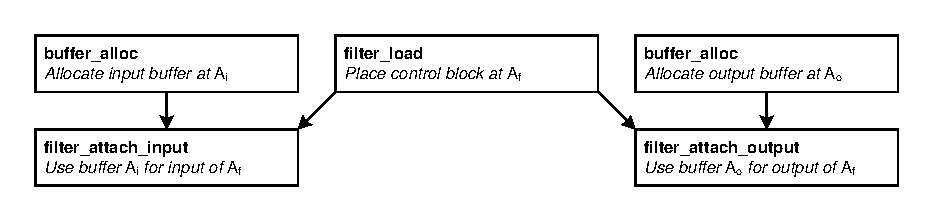
\includegraphics[scale=.55]{figs/init}
\end{center}
\caption[Commands to set up a filter.]{Commands to load a filter and allocate and attach input and output buffers. Lines between commands represent dependencies that must be specified to the library when the commands are issued. These commands may be issued in one or multiple groups.}
\label{fig:lib:init}
\end{figure}

In addition, input data must be transferred into the input buffer before the filter can be run, and output data must eventually be transferred out of the output buffer. With an initially empty input buffer, the commands to transfer in $n$ iterations of input, run the filter for $n$ iterations, and then transfer out $n$ iterations of output (assuming that the input and output buffers were sized appropriately) are shown in Figure~\ref{fig:lib:run}.

\begin{figure}[!htb]
\begin{center}
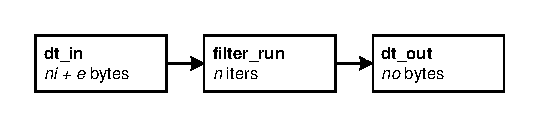
\includegraphics{figs/run}
\end{center}
\caption[Commands to run a filter.]{Commands to run a filter for the
  first $n$ iterations, including transferring input and output. The
  corresponding data transfer commands on other cores are not shown.}
\label{fig:lib:run}
\end{figure}

A sequence of commands is required to run the filter for a larger
number of iterations on a core with a finite local store
capacity. This is illustrated in Figure~\ref{fig:lib:ext}.

\begin{figure}[!htb]
\begin{center}
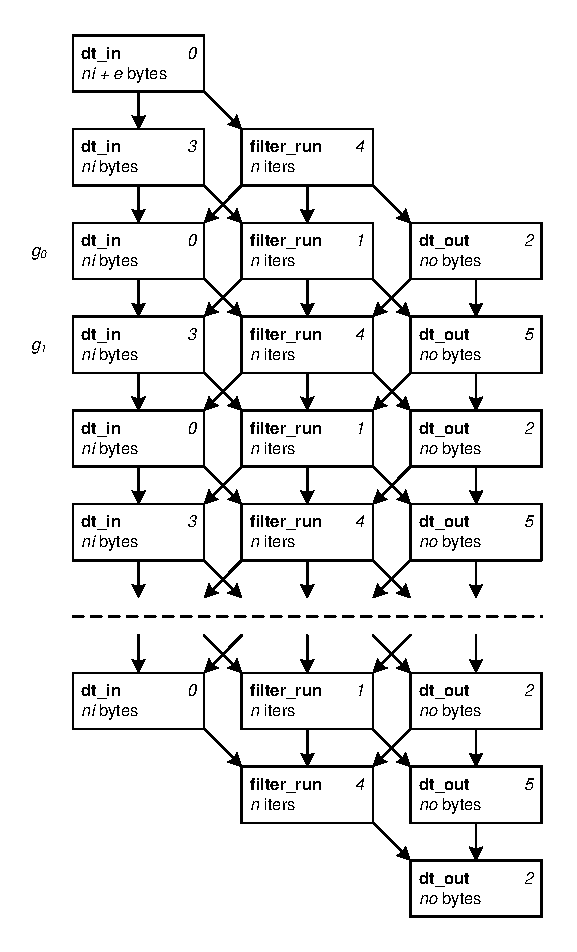
\includegraphics[scale=.90]{figs/ext}
\end{center}
\caption[Sequence of commands to run a filter for a large number of iterations.]{Sequence of commands to run a filter for a large number of iterations. Command IDs are indicated in the upper right. Each row is issued as a different group.}
\label{fig:lib:ext}
\end{figure}

Provided that the input buffer is at least $2ni+e$ bytes and the output buffer is at least $2no$ bytes, the dependencies among the commands in the sequence ensure that:
\begin{itemize}
\item When a \textsf{dt\_in} command becomes active, there are at most $ni+e$ bytes of data in the input buffer, and thus enough space to transfer in an additional $ni$ bytes.
\item When a \textsf{dt\_out} command becomes active, there are at least $no$ bytes of data in the output buffer, and thus enough data to transfer out.
\item When a \textsf{filter\_run} command becomes active, there are at least $ni+e$ bytes of data in the input buffer and at most $no$ bytes of data in the output buffer. This is enough input data and output space to run the filter for $n$ iterations.
\end{itemize}

This sequence of commands effectively ``pipelines'' the basic operation from Figure~\ref{fig:lib:run}. Double-buffering is accomplished when the data transfer commands in a group complete before the \textsf{filter\_run} does. In this case, the following \textsf{filter\_run} has no outstanding dependencies once the current \textsf{filter\_run} completes, and can become active immediately.

The user or scheduler can keep the core continually supplied with work
by initially issuing the first two groups, thereafter issuing the next
group whenever a group completes. In this case, the core almost always
has two groups of commands issued, with one group active and the other
queued. In addition, with the exception of the first two and last two
groups, the command parameters, IDs and dependencies in every other
group are identical. This allows the user to initially set up two
groups ($g_0$ and $g_1$ in Figure~\ref{fig:lib:ext}) and repeatedly
issue them for a majority of the execution. If executions are
relatively long, the overhead of the first and last group, where no
filter is being run, will be amortized effectively. Alternatively, the
user can load another filter and run it during those gaps.

In practice, situations such as the above, where a static-rate filter
is run for a large number of iterations and large amounts of input and
output data are transferred, are very common in streaming code. To
avoid requiring the user to manually issue groups and deal with
command completion callbacks in every such case, the MSL library also
provides extended operations that encapsulate this pattern. In an
extended operation, the user provides the library with filter rates,
the addresses of opposing buffers on other processors for data
transfers, and the number of groups to run for; the library issues and
responds to all commands internally and notifies the user when the
entire operation is complete.
%% Where one or both opposing buffers are located in memory,
%% the library also handles the PPE side of data transfers
%% internally. 
Extended operations greatly simplify setting up pipelines
of any length where all filters in the pipeline have static rates.


%\section{Implementation}

Filters that use induction variables inherently use state to keep track of
how often it has been called through the span of the program.  We attempt 
to remove this user-facing state by introducing an iteration keyword to the 
StreamIt language.  Functionally, this iteration keyword returns how often 
the work function of the corresponding filter has been called.  Filters 
using this feature are no longer classified as stateful in the StreamIt
compiler, as the compiler has the means of fissing these filters in a 
predictable manner.

In translating higher level code into the intermediate representation, the 
iteration keyword is desugared.  The compiler adds an internal induction 
variable field for filters that use the iteration keyword.  This induction
variable is incremented at the end of each \texttt{work} call.  Any instance
of the iteration keyword is translated into a reference to this internal 
induction field.  

This desugaring process introduces induction variable state to the intermediate
representation of the filters.  Modifications must also be made to the fission 
process to allow the compiler to fiss these stateful filters and ensure 
consistency between fission products after fission.  

The fission process now modifies the fission products by adding the 
following values as fields of the products:
\begin{itemize}
	\item \texttt{start}: the value of the induction variable each product starts with.
	\item \texttt{reps}: how often the \texttt{work} function of the product is 
	  called between rounds.
	\item \texttt{total}: the sum of all reps of all fission products. This value is 
	  the same amongst all fissed products.
\end{itemize}
Accordingly, each fission product should start each round with induction values
of
\begin{center}
\texttt{total}*\texttt{n} + \texttt{start}
\end{center}
and range up to the value
\begin{center}
\texttt{total}*\texttt{n} + \texttt{start} + \texttt{reps} - 1
\end{center}
where \texttt{n} is a nonnegative integer indicating how many rounds have
been run in the span of the program.  We have to account for the off-by-one
error as the first iteration is run.

At the end of each fission product \texttt{work}, after incrementing the 
induction value, a check must be made to see if it is necessary to increment 
the induction variable to the next round of  values.  This will prevent certain
fissed products from making calls with duplicate induction values.  
\begin{center}
\texttt{iter} - \texttt{start} - \texttt{reps} \% \texttt{total} == 0
\end{center}
The fissed products must check that the current induction value less the 
\texttt{start} and \texttt{reps} of that fissed product is divisible by the 
\texttt{total}.  This is consistent with the maximum value per round as 
indicated above.  Once the fissed product's induction value has reached 
this value, it must be set to:
\begin{eqnarray*}
\texttt{iter}_{n+1} &=& \texttt{iter}_{n} + (\texttt{total} - \texttt{reps}) \\
&=& (\texttt{total}*\texttt{n} + \texttt{start} + \texttt{reps}) \\
&&  \ \ +\ (\texttt{total} - \texttt{reps}) \\
&=& (\texttt{total}*(\texttt{n+1}) + \texttt{start})
\end{eqnarray*}
which is the starting iteration value of the next round, as defined.

The scheduler may also modify the multiplicity of the rounds.  The field values
added to the fissed products must, in turn, be updated to reflect this change.
Since all fissed products will be multiplied by the same steady multiplicity
factor, we can simply multiply each of the \texttt{start}, \texttt{reps}, and 
\texttt{total} values by the same steady multiplicity value.



%\section{Mapping StreamIt Patterns to the Runtime Library}\label{ch:use}

There are a number of common execution patterns that can be used to run a StreamIt program (see section~\ref{ch:bg:str:exec}). To illustrate how these patterns can be mapped to the runtime library for Cell, we will refer to the FFT StreamIt benchmark as a concrete example. This program performs a 256-element fast Fourier transform. The program's stream graph consists of a single pipeline of 15 filters. Every filter in the pipeline is stateless (and hence data-parallel) and does not peek. A single complete execution of the stream graph processes a single set of 256 input elements (512 floats), producing the same number of output elements.

%% \begin{figure}[!htb]
%% \begin{center}
%% 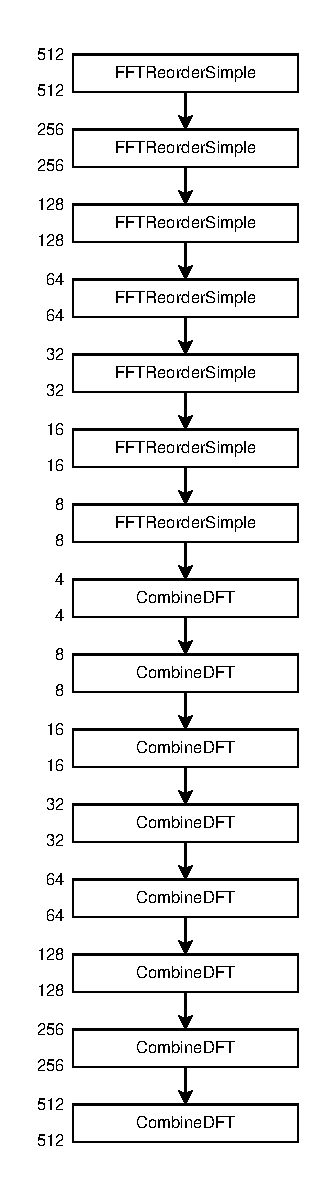
\includegraphics{figs/fftgraph}
%% \end{center}
%% \caption[Stream graph for 256-element FFT.]{Stream graph for 256-element FFT. A single execution of the stream graph pops and pushes 512 floats, since each element is a complex number whose components are interleaved on tapes.}
%% \label{fig:use:fftgraph}
%% \end{figure}

Data-parallel filters are the simplest to map to the library. The entire FFT pipeline can be fused into a single data-parallel filter that pops and pushes 512 floats per work function iteration. The fused filter can be data-parallelized over many SPEs: pseudocode to do this is illustrated in figure~\ref{fig:use:dp}. The \textsf{ext\_ppu\_spu\_ppu\_ex} library function starts an extended operation that loads the filter, allocates its buffers, and runs it for a large number of iterations.\footnote{The user still specifies all major parameters -- for example, the addresses to allocate buffers at and how many iterations each \textsf{filter\_run} command runs for.} The line containing \textsf{spulib\_poll\_while} synchronizes all SPEs; it returns only when all SPEs have finished and the callback has been run for each SPE.

\begin{figure}[!htb]
\begin{center}
\begin{tabular}{ll}
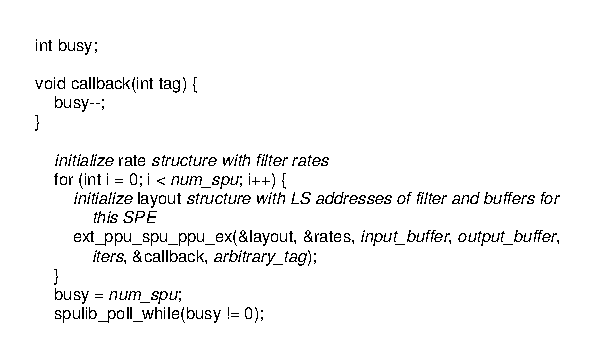
\includegraphics{figs/dpcode} & 
\includegraphics{figs/dp}
\end{tabular}
\end{center}
\caption[Pseudocode for running a data-parallel filter.]{Pseudocode for running a data-parallel filter. The figure on the right represents the state of each SPE as time passes. The horizontal line indicates synchronization by the PPE.}
\label{fig:use:dp}
\end{figure}

Course-grained software pipelining~\cite{asplos06} can be implemented similarly. Typically, the user will have assigned each filter in the steady state to an SPE and allocated and populated a buffer in memory for each channel. Pseudocode to execute a single iteration of the steady state is illustrated in figure~\ref{fig:use:swpipe}. Again, the line containing \textsf{spulib\_poll\_while} synchronizes all SPEs; this is necessary to ensure that sufficient input data has been produced for every filter in the next steady state iteration. For efficiency, the steady state should be sufficiently coarsened to amortize the overhead while SPEs are switching between filters and thus not performing any computation.

\begin{figure}[!htb]
\begin{center}
\begin{tabular}{ll}
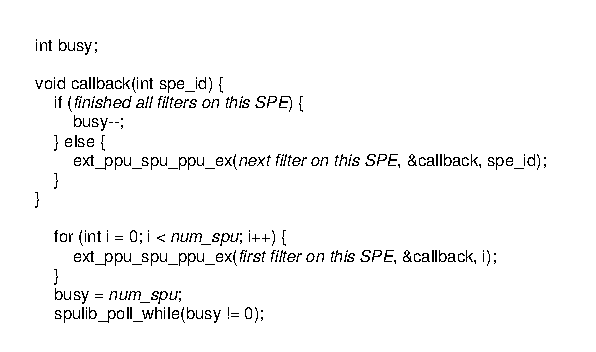
\includegraphics{figs/swpipecode} & 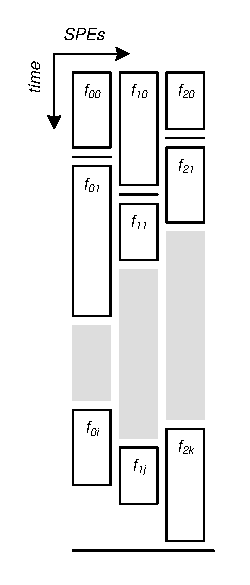
\includegraphics{figs/swpipe}
\end{tabular}
\end{center}
\caption[Pseudocode for running a course-grained software pipeline.]{Pseudocode for running a course-grained software pipeline. The figure on the right represents the state of each SPE as time passes. Horizontal lines indicate synchronization by the PPE.}
\label{fig:use:swpipe}
\end{figure}

Both patterns presented so far involve no direct SPE--SPE communication. An alternative implementation for FFT partially fuses the 15 filters in the StreamIt pipeline into a number of library filters, which are simultaneously run on different SPEs. These SPEs can transfer data between local stores directly, taking advantage of Cell's on-chip communication network and avoiding the extra latency to memory, as well as preventing memory from possibly becoming a bottleneck. Pseudocode to do this is illustrated in figure~\ref{fig:use:spepipecode}.

%% \begin{figure}[!htb]
%% \begin{center}
%% 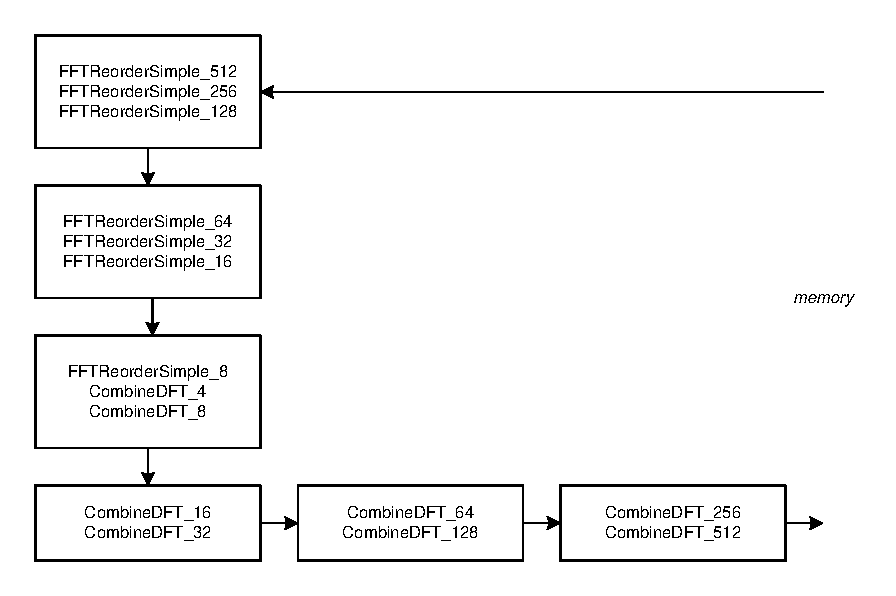
\includegraphics{figs/spepipe}
%% \end{center}
%% \caption{Pipelining FFT over six SPEs.}
%% \label{fig:use:spepipe}
%% \end{figure}

\begin{figure}[!htb]
\begin{center}
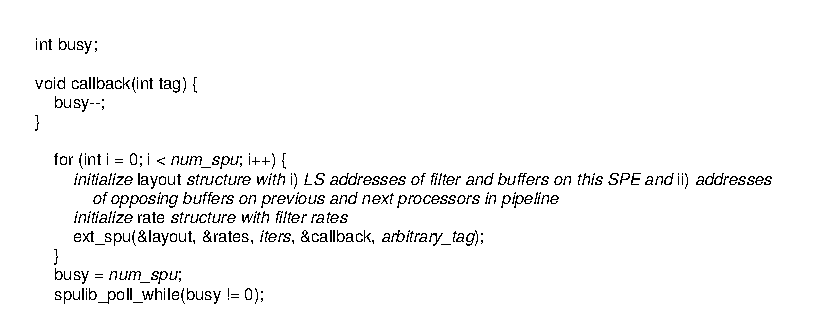
\includegraphics{figs/spepipecode}
\end{center}
\caption{Pseudocode for setting up an SPE--SPE pipeline.}
\label{fig:use:spepipecode}
\end{figure}

More complex scheduling choices require the user to provide more complex callback functions. For example, the communication overhead of loading a new filter onto an SPE can be hidden if the load is performed while the old filter is still running its last iterations.

The library allows the user to treat filters as individual schedulable entities, instead of having to consider complex lower-level operations. The pseudocode in figure~\ref{fig:use:dp} can be compared to the SPE code required to execute the same pattern (a single fused data-parallel filter) without using the library, illustrated in figure~\ref{fig:use:handcode}.

\begin{figure}[!htb]
\begin{center}
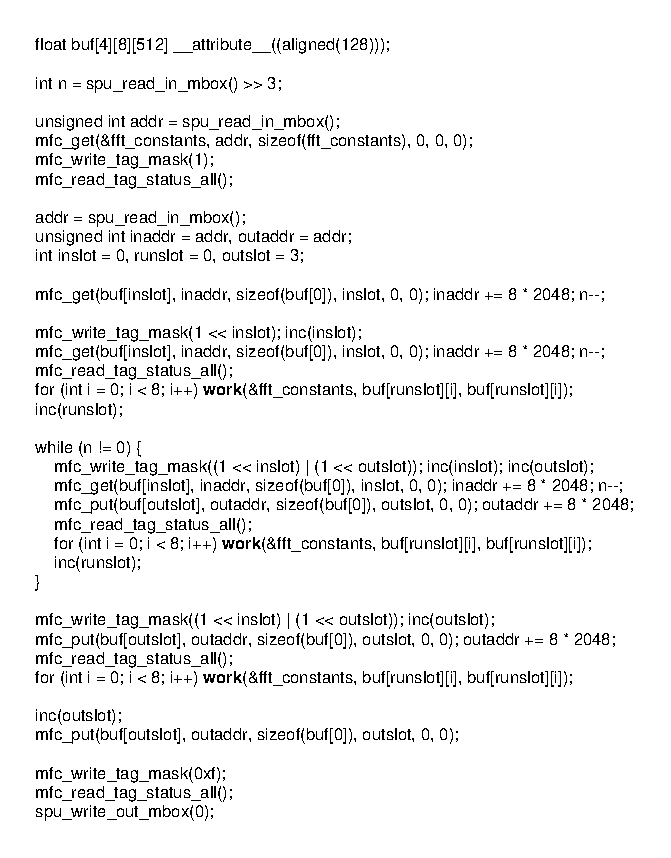
\includegraphics{figs/handcode}
\end{center}
\caption[SPE code for hand-coded implementation of data-parallel fused FFT.]{SPE code for hand-coded implementation of data-parallel fused FFT. The three bolded calls to \textsf{work} actually run the fused work function; the rest of the code performs double-buffered data transfers.}
\label{fig:use:handcode}
\end{figure}

This code is not overly complex, and will always be more efficient than using the library. However, this code is also specific to the filter and the execution pattern. The fused filter in FFT does not peek, and conveniently produces and consumes amounts of data that are compatible with Cell's DMA alignment requirements. The code would have to be significantly changed if a filter with slightly different rates were substituted. If multiple filters need to be run on an SPE, the code would then acquire additional logic to switch between filters. To run filters in an SPE--SPE pipeline, additional code would be needed to synchronize between SPEs. Using the library, the user does not need to deal with any of this.

\section{Splitters and Joiners}

In general, the type of fine-grained data reorganization performed by round-robin splitters and joiners cannot be directly implemented using Cell's DMA mechanism, which has strict alignment requirements. However, since the library supports filters with multiple input and/or output tapes, a compiler can simply define separate filters for each splitter and joiner. A compiler can also fuse a splitter or joiner with the upstream or downstream filter, respectively; the resulting filter has a much lower communication--computation ratio than an independent splitter or joiner.

The user can ignore duplicate splitters as long as the output of the upstream filter is buffered into memory. Because multiple PPE buffers can refer to the same data region, no duplication of data in memory is necessary. However, if the filters downstream of the splitter run on different SPEs, the same data must be copied to the local store of each SPE.

\section{Scheduling Stream Programs Using the MSL}\label{ch:ds}

Streaming programs typically allow for a lot of freedom in terms of
orchestrating the parallel execution of the stream graph. This freedom is
afforded by the dataflow models of computation that many streaming
languages are founded on. In a stream program, the rules governing the
execution of a node or actor in the graph are often simple, and usually
reduce to having sufficient buffering on the input to an actor, and
sufficient buffering to store the output.

The execution of a stream program requires mapping and ordering actors
to cores, allocation of buffers, and managing data transfers between
buffers. Collectively, mapping, ordering, and buffer managements are
embodied in a schedule of execution.

It is possible to devise a schedule statically (e.g., compile time or
at graph creation time) or dynamically (e.g., runtime). The goal of a
scheduler is simply to maximize the throughput of the streaming
application. In the age of multicore architectures, a scheduler will
need to utilize multiple cores to increase concurrency and hence improve
the throughput of a given streaming application. 

A dynamic scheduler is conceptually easy to understand. The scheduler
maintains an internal representation of a given stream graph (e.g.,
list or priority queue). In a multicore architecture, when there is a
core available, the scheduler scans its internal representation of the
stream graph, and determines which actor is ready to fire.
The scheduler assigns the actor to the available core. The core is
also informed where the input buffer for the actor resides in memory,
and where in memory to commit (buffer) the output of the actor for its
successors. The scheduler then updates its internal representation to
indicate the actor firings and implement a fairness policy to assure
overall progress (e.g., a round-robin scheduler).

For stream graphs that are ``predictable'', dynamic scheduling
generally does not present any advantages over static
scheduling. Dynamic scheduling inevitably involves additional
communication and scheduling overhead due to extra filter loading and
unloading, buffer management, and scheduling computation. When all
filters in a program are data-parallel, a static scheduler can make
full use of all cores by simply executing each filter in turn on all
cores, with a sufficient coarsening of the steady state to amortize
filter load/unload and synchronization overhead. The optimal
situation results when the compiler can fuse all filters into a single
data-parallel filter; this produces the minimum possible communication.
This situation would also be optimal for a dynamic scheduler.

Even when filters are stateful and thus cannot be data-parallelized,
static software pipelining techniques~\cite{asplos06} can make full
use of cores when the compiler has an accurate static work estimator
and can divide filters in a steady state evenly across
cores. A single stateful filter with a heavily imbalanced work
function creates a bottleneck, but dynamic schedulers are also faced
with this problem. 
%%In addition, no ``unpredictable'' cache misses or
%%lengthy communication delays that can skew a static work estimate are
%%possible on the Cell architecture.

Dynamic scheduling becomes beneficial when filters are not
``predictable'': when it is difficult to statically balance load
across cores, difficult to estimate the amount of work done by filter
work functions, or work functions perform widely varying amounts of
work through the execution of the program. In these situations,
dynamic scheduling may be able to deliver better load-balancing than
static scheduling.

A dynamically scheduled program can be run on varying numbers of
processors without requiring recompilation or the reanalysis that
complex static schedulers would need to perform, and is also tolerant
of changes in the availability of processors while the program is
running. 
%% In addition, for stream graphs that contain filters with
%% dynamic rates, it may not be possible to statically predict how many
%% times filters will be run, and the balance of work in the stream graph
%% may change as the program is run. In this case, only dynamic
%% scheduling is able to shift workload to different portions of the
%% stream graph as needed.\footnote{However, the current dynamic
%% scheduler implementation does not support dynamic rates.}

%% \section{User Interface}\label{ch:ds:ui}

%% The user provides as input to the dynamic scheduler a complete
%% description of the stream graph, specifying filters and the
%% channels that connect them. Rates for all filters must be
%% specified. Duplicate splitters can be handled by setting parameters
%% of channels; round-robin splitters and joiners must be defined as
%% separate filters.

\subsection{Methodology}

We evaluated dynamic and static scheduling schemes for the Cell
multicore architecture. The Cell processor has 9
cores~\cite{Cell-hpca}: a PPE that serves as a general purpose
processor, and 8 SPEs that are designed to perform the bulk of the
computation. Each SPE has 256KB of local store and a DMA processor to
manage data in and out of the SPE. In our methodology, the schedule is
run on the PPE and the filters run on the SPEs.

We used the StreamIt~\cite{streamitweb} programming language to
generate the stream graph that is presented to the MSL and to both the
static and dynamic schedulers. The basic unit of computation in StreamIt is a 
{\it filter}. There are three basic constructs for composing filters
into a communicating network: a {\it pipeline}, a {\it splitjoin}, and
a {\it feedbackloop}. A pipeline behaves as the sequential composition
of all its child streams. A splitjoin is used to specify independent
parallel streams that diverge from a common {\it splitter} and merge
into a common {\it joiner}. A feedbackloop provides a way to create
cycles in the stream graph.

\subsection{Static Scheduler Implementation}

The Cell backend for the StreamIt compiler maps StreamIt programs to C code that
is run on the Cell processor through the MSL. The backend 
is built upon the robust StreamIt compiler infrastructure~\cite{asplos06}. 
Briefly, StreamIt code is converted into a
high-level stream IR which then undergoes a series of optimizing transformations.

In the case of static scheduling, the compiler processes the stream program
through four phases.
\begin{itemize}
\item In the scheduling phase, a steady state schedule, which maintains a constant
number of data items in each input and output buffer after every execution, is calculated based on each
filter's declared I/O rates. This steady state schedule can then
be run in an infinite loop. Additionally, an initialization schedule may be
generated to prime the buffers or initialize state.
\item In the partitioning phase, filters are fused or
fissed to achieve the best level of granularity for the best load balancing.
\item In the layout phase, filters are assigned to specific cores on which
they are run.
\item In the code generation phase, appropriate code that encapsulates the schedule,
partitioning, and layout are generated and run on the target architecture.
\end{itemize}

For our data parallel applications, our partitioning
phase fuses all filters into a single filter. We generate all code, both control and
filter work function code, through the backend. We then run this fused filter
in parallel across all SPEs. Many real-world applications are stateless and can
therefore be data-parallelized in this fashion.

%For MPEG2, we isolated the stateful filter and fused all other stateless filters.
%We then profiled these two filters to find a schedule that provides good load balancing
%between SPEs. We generate the work function code through the backend, but hand-coded
%the control code on the PPE.


\subsection{Dynamic Scheduler Implementation}\label{ch:ds:imp}

The Cell architecture's communication network provides very high
memory bandwidth. The design of the dynamic scheduler assumes that
memory bandwidth will never be a bottleneck, and the dynamic scheduler
buffers all output produced on SPEs to memory. The scheduler performs
dynamic course-grained software pipelining on the stream graph; if
sufficient data can be buffered in all channels at all times, pipeline
stalls can be avoided and all SPEs can be fully utilized. While
SPE--SPE communication is more efficient than SPE--memory
communication, SPE local store is generally too limited to store the
buffering needed for software pipelining, and thus the scheduler never
executes SPE--SPE pipelines; this avoids having to deal with work
imbalances between pairs of adjacent filters. At any time, any two
SPEs will typically be operating on data from different 
iterations of the program.

At startup, the dynamic scheduler allocates a large\footnote{1 MB in
the current implementation, but this can be adjusted.} buffer in
memory for each channel; this is used to buffer the output of the
upstream filter to provide input for the downstream filter. At any
time, for any specific filter, the amount of data available in its
input channels and amount of space available in its output channels,
along with its rates, determines the maximum number of iterations that
the filter can be run for.

The scheduler selects filters to run on SPEs based on a metric
computed from the maximum number of iterations and certain filter
properties (see below). When a filter is selected to run on an SPE, it
is scheduled for a limited but fairly large number of iterations in
order to amortize the cost of loading it. Filters run for their entire
allotment of iterations; however, allotments are kept small to allow
the scheduler to quickly schedule another filter if necessary in
response to the changing amount of data in different parts of the stream graph.

Using command completion notifications,
the scheduler determines when the current filter scheduled on an SPE has
almost finished running for all of its allotted iterations and selects
a replacement filter for the SPE.
While the current filter is still running, the
scheduler issues additional commands to load the new filter, allocate
its buffers, and transfer data into its input buffers from memory;
this communication is overlapped with the computation done by the
current filter. When the replacement filter is the same as the current
filter, this additional work can be avoided. Finally, the first
command to run the new filter is queued after the last command to run
the current filter. When the replacement filter is selected early
enough, it will be set up on the SPE before the current filter
finishes running, ensuring that it can start running as soon as the
current filter finishes. When the current filter has completed all of
its allotted iterations, it is unloaded and can then be scheduled on
another SPE.

The dynamic scheduler can run multiple instances of data-parallel
filters on multiple SPEs at the same time. A data-parallel filter is
still selected by the same metric as other filters; it will only be
run on more than one SPE at once if it is determined to be significantly better than
other filters.

The current metric implemented is very simple: it prioritizes filters
based on the amount of data the state of their input and output
channels allow them to consume and produce, respectively. However, the
filter that is currently running on an SPE is prioritized when
considered for scheduling on the same SPE; this effectively causes
filters to be run for as long as possible on an SPE, with no load
overhead, while no other filters are significantly better. Other more
complex metrics can be easily substituted. We have yet to make a
full analysis of the design of metrics and their effects on the propagation
of data through the stream graph; we plan to use the dynamic scheduling
framework to investigate this.

When the dynamic scheduler encounters a pipeline, the filter selection
metric quickly causes all filters in the pipeline to be run
sufficiently to generate some data in every channel
buffer. Thereafter, the sequence of filter executions selected by the
scheduler appears to perform software pipelining, although without a
recognizable steady state.

\subsection{Code Generation}

%Following the previous phases, code generation is the final phase in the StreamIt
%compiler. One option is to generate code directly targeting the Cell API.
%The disadvantages of this approach include the additional burden of
%dealing explicitly with DMA alignment requirements and the bloated code. Here,
%the library provides a convenient layer of abstraction which not only abstracts
%away DMA transfers but also provides for code that is more readable and easier
%for the compiler to generate.
For both static and dynamic scheduling cases, we must generate the code that
is to be run on the multicore. In the case of Cell, we generate C
code that utilizes the library and compile it with Cell's GCC. We run all
control code on the PPE and all filter initialization and work functions on the SPEs. 

We set up filter description parameters
specifying how many inputs and outputs a filter has, which input and output
buffers the filter reads from and writes to, and how many bytes the filter 
reads and writes in one execution. These parameters are then used by the
library to handles the necessary data transfers and executions of the
work function of the filter. 

In the case of dynamic scheduling, scheduling, partitioning, and layout
are handled at run-time by the dynamic scheduler. Thus, the compiler need only
generate the aforementioned code to set up the scheduler for execution.

In the case of static scheduling, we additionally set up filter layout parameters
which specify on which SPE a filer should be run. The init and steady state
schedules are explicit in the code: filters are loaded and run according to the
schedule, and callbacks are used to set up parameters for and to run the next filter in
the schedule.

\section{Performance}\label{ch:perf}

We evaluate the performance of the MSL library and StreamIt compiler backend
on a set of four StreamIt applications using different scheduling
methodologies. The applications are described in figure~\ref{fig:perf:apps}.
For statically-scheduled benchmarks, the scheduler executes a sufficiently
coarsened steady state to reduce library overhead and imposes an explicit
synchronization barrier between steady state iterations. The dynamic scheduler
automatically coarsens work functions as necessary.

\begin{figure}[!htb]
\begin{center}
\begin{tabular}{|l|p{2.25in}|}
\hline
BitonicSort & 8-element bitonic sort \\
\hline
DCT & 16x16 IEEE reference DCT \\
\hline
FFT & 256-element FFT \\
\hline
MPEG & MPEG-2 block and motion vector decoding (subset of full MPEG-2 decoder) \\
\hline
\end{tabular}
\end{center}
\caption{Benchmark applications.}
\label{fig:perf:apps}
\end{figure}

The benchmarks were executed on PlayStation 3 hardware, which only provides
six usable SPEs. Benchmarks were run for a large number of steady state
iterations to smooth out any one-time execution startup overhead.
Performance numbers are given in Figure~\ref{fig:perf:stats}.

\begin{figure}[!htb]
\begin{center}
\begin{tabular}{|l|r|r|r|r|}
\hline
& Cores & Run~\% & Work~\% & GOPS \\
\hline
\textsf{BitonicSort\_static} & 6 & 98.2 & 97.8 & 0.5 \\
\hline
\textsf{DCT\_static} & 6 & 98.5 & 97.5 & 3.2 \\
\hline
\textsf{FFT\_static} & 6 & 99.0 & 98.4 & 1.9 \\
\hline
\textsf{FFT\_dynamic} & 6 & 99.3 & 89.8 & 2.2 \\
\hline
\textsf{FFT\_pipeline~*} & 6 & 95.9 & 92.2 & 1.9 \\
\hline
\textsf{MPEG\_static~*} & 5 & 98.2 & 97.7 & N/A \\
\hline
\textsf{MPEG\_dynamic} & 5 & 98.8 & 96.9 & N/A \\
\hline
\end{tabular}
\end{center}
\caption{Benchmark performance.}
\label{fig:perf:stats}
\end{figure}

The \emph{Cores} column gives the number of SPEs each benchmark is
scheduled for and run on. Utilization statistics are maintained by the
MSL library. The \emph{Run~\%} column gives the percentage of total time the SPE had an active \textsf{filter\_run} command. The remainder is overhead due to either \emph{i}) durations when SPEs do not have useful work to do (such as when waiting for filters to be loaded) or \emph{ii}) inadequate double-buffering of input or output data. In both cases, the scheduler (or the nature of the program) creates insufficient communication--computation concurrency. The \emph{Work~\%} column gives the percentage of total time actually spent in the work function. The remainder represents the total overhead added by the library or caused by the scheduling algorithm.
The Run~\% and Work~\% numbers given for each benchmark are for the SPE
that reported the greatest work percentage.
For \textsf{DCT} and the FFT benchmarks, the \emph{GOPS} column gives GFLOPS.
For \textsf{BitonicSort}, the \emph{GOPS} column gives billions of
compare operations per second.

The \textsf{FFT\_pipeline} and \textsf{MPEG\_static} benchmarks (indicated
with a \textsf{*} in the figure) exhibit behavior that is not adequately
described by the statistics alone, which we discuss below.

The \textsf{BitonicSort}, \textsf{DCT}, and \textsf{FFT} benchmarks are statically-scheduled and generated by the StreamIt compiler. These application are fully data-parallel and the compiler fuses the stream graph into a single filter. This is then split to the number of cores. 
As the number of SPEs is varied from one to six, utilization numbers remain nearly the same. Utilization and runtimes are always nearly identical across all SPEs. This demonstrates nearly perfectly linear speedup.
From Work~\%, the overhead added by the library is less than 2.5\%. Run~\% is high, although not exactly 100\% due to the overhead of starting each steady state and the synchronization barrier after each steady state.

For a single fused data-parallel filter, the dynamic scheduler provides identical performance as static scheduling. Results for the dynamic scheduler on these applications are not separately given.

The \textsf{FFT\_dynamic} and \textsf{FFT\_pipeline} benchmarks are different manual implementations of the FFT application. The FFT stream graph consists of a single pipeline with 15 filters. \textsf{FFT\_dynamic} schedules this pipeline using the dynamic scheduler. In \textsf{FFT\_pipeline}, the stream graph is first manually fused into a pipeline of six filters, each of which is statically placed on a different SPE. All communication except for input and output is done directly between SPE local stores and remains entirely on-chip. GFLOPS numbers for \textsf{FFT\_dynamic} and \textsf{FFT\_pipeline} can be compared with each other but not directly to \textsf{FFT}; the former two have manual work function implementations that are slightly more efficient than the compiler-generated code.

For \textsf{FFT\_dynamic}, utilization and runtimes are nearly identical across all SPEs and Run~\% is very close to 100\%. This indicates that the dynamic scheduler has no difficulties keeping all SPEs supplied with work. Moreover, it validates the critical assumption made in the design of the dynamic scheduler: the Cell architecture's memory bandwidth is indeed sufficient to perform all buffering to memory, avoiding SPE--SPE communication entirely. Utilization numbers remain nearly identical as the number of SPEs is varied from one to six, indicating almost perfectly linear speedup. 

However, Work~\% shows that this benchmark has approximately 10\% overhead. From the high Run~\%, almost all of this is due to the library. This overhead results from two factors: \emph{i}) individual filters in the pipeline have much lower communication--computation ratios than the single fused filter in the \textsf{FFT} benchmark; and \emph{ii}) the dynamic scheduler continually issues additional commands to switch filters between SPEs which are not needed in a static schedule.

For \textsf{FFT\_pipeline}, a single filter/SPE in the middle of the pipeline is the bottleneck. Although GFLOPS is 12\% lower than \textsf{FFT\_dynamic}, no SPE except for the bottleneck was fully utilized: two other SPEs had Work~\% around 60\%. In general, this illustrates the difficulty of performing direct static SPE--SPE pipelining. Although SPE--SPE pipelining keeps communication on-chip, where extremely high bandwidth is available and there is no danger of exhausting comparatively limited memory bandwidth, work imbalances between filters make it difficult to fully utilize all SPEs.

MPEG has a small amount of state and cannot be fused into a single filter. The compiler fuses the stream graph down to a single stateful filter and a single stateless filter as the branches of a two-way splitjoin. For mapping to the MSL library, both statically- and dynamically-scheduled benchmarks explicitly treat the scattering and gathering operations as separate stateless filters, resulting in a total of four filters to schedule.

The \textsf{MPEG\_static} benchmark statically software-pipelines these four filters. We generated a static schedule for five SPEs by manually profiling, splitting, and partitioning filters and manually generating control code to issue the resulting schedule. The mapping of filters to SPEs in the partition that we obtained is given in Figure~\ref{fig:perf:mpegs}.

\begin{figure}[!htb]
\begin{center}
\begin{tabular}{|r|l|}
\hline
SPE & Filters \\
\hline
0 & $n$ splitter, $n$ stateful \\
\hline
1 & $6n$ joiner \\
\hline
2 & $2n$ stateless \\
\hline
3 & $2n$ stateless \\
\hline
4 & $2n$ stateless \\
\hline
\end{tabular}
\end{center}
\caption{Partition for \textsf{MPEG\_static} benchmark.}
\label{fig:perf:mpegs}
\end{figure}

This partition has a slight work imbalance. The Run~\% and Work~\% numbers given in figure~\ref{fig:perf:stats} are for SPEs~2--4, which have the highest utilization. SPE~0 has the lowest utilization (88.3\%). However, aside from the work imbalance, which can be minimized with a better partition, this benchmark shows that static software pipelining using the MSL library can be done with very low overhead.

The \textsf{MPEG\_dynamic} benchmark uses the dynamic scheduler to schedule the four filters. 
As with \textsf{FFT\_dynamic}, utilization and runtimes are nearly identical across all SPEs and there is nearly perfectly linear speedup as the number of SPEs is varied. Compared to the static schedule, the dynamic scheduler is not limited by the concept of a steady state and does not impose any synchronization barriers; however, in order to dynamically switch filters on cores, it must issue more commands. This translates into slightly higher Run~\% but slightly lower Work~\%. However, the dynamic scheduler is able to more efficiently distribute work across all available cores; overall, this results in a 2.5\% performance improvement over \textsf{MPEG\_static}.

The performance of the benchmarks in terms of GOPS is relatively low compared
to the theoretical maximum performance. One contributing factor to these
results is the fact that no SIMD vectorization was performed. For these
benchmarks, vectorization has potential to significantly increase performance.
Nevertheless, we believe that the high utilization achieved is the major
contribution.
\section{Related Work}
\label{sec:related}

Software pipelining for clustered vliws \cite{qian02}.

The Imagine stream processor~\cite{rixner98bandwidthefficient}
supports a time-multiplexed execution model.  The architecture
contains 48 parallel ALU's organized into 6 VLIW clusters.  The
programming model requires the programmer to write computation filters
in Kernel-C and stitch them together using Stream-C.  Because the
execution unit is data-parallel, the compiler uses time multiplexing
to execute a single filter at a time across all of the parallel
clusters.  While this provides perfect load balancing and high
arithmetic utilization when there is abundant data parallelism, it
suffers when a filter has retained state or data-dependences between
iterations.  Moreover, architectures based solely on
time-multiplexing do not scale spatially, as there are global wires
orchestrating the parallel execution units. 

Previous work in compiling StreamIt to Raw has taken a purely space
multiplexed approach~\cite{streamit-asplos}.  In this model, a single
filter was mapped to each execution tile.  To support applications
with more filters than execution tiles, a partitioning algorithm was
employed to adjust the granularity of the graph by fusing adjacent
filters into one.

Previous work in scheduling computation graphs to parallel targets
have focused on dynamic techniques \cite{SDFSched, SDFSched2,
may87communicating, DAGSched}. In general, multiple graph nodes are
{\it clustered} onto a single computational node and scheduled
dynamically.  

Our work, unlike most previous work in this field,
models link contention and topography.  Furthermore, StreamIt graphs
are implicitly formed of loops so we can apply loop scheduling
techniques such as software pipelining to build our schedules.

%The problem of instruction scheduling for MIMD and VLIW architectures
%is similar to the problem tackled by the space-time compiler.  ILP
%compilers for clustered VLIW architectures~\cite{Bulldog, Multiflow}
%are decomposed into stages that are analogous to the stages of the
%SpaceTime compiler.  These compilers must partition or cluster
%instructions, assign instructions to processors, and then schedule the
%instructions.  

Previous work on software pipelining has focused on scheduling machine
instructions in a loop \cite{lam-softpipe, rau-softpipe} to a
uniprocessor target.  The algorithms devised must account for tight
resource constraints and complex instruction dependences.  Our
software-pipelining problem is much less constrained, a traditional
modulo scheduling algorithm can not effectively take advantage of this
flexibility.  Previous work on ILP scheduling for the Raw
architectures ~\cite{lee98spacetime} also bears similarity.  However,
these compilers schedule graphs of fine-grained instructions. The
partitioning and scheduling heuristics are mindful of a different set
of constraints including different types of dynamism and less regular
communication patterns as compared to StreamIt graphs.

As far as we know, we are the first to apply loop-level scheduling
techniques to the problem of scheduling coarse-grained task graphs.

% \cite{cheops-thesis}
%   http://web.media.mit.edu/~kung/publication/thesis.pdf
%
% other possible things to cite:
%  http://portal.acm.org/citation.cfm?id=801721&dl=ACM&coll=portal
%  http://www.csrl.unt.edu/~kavi/Research/ica3pp156.pdf
%  http://cdmetcalf.home.comcast.net/papers/cop/node1.html#SECTION00010000000000000000

\section{Conclusions}\label{ch:conc}

Streaming languages such as StreamIt provide an excellent way to target new multicore architectures while placing minimal parallelization burden on the programmer. The Cell architecture is designed to offer high peak performance, and is very suited for streaming applications. This thesis described a runtime framework for streaming applications on Cell consisting of \emph{i}) a runtime library that provides high-level primitives for schedulers and \emph{ii}) a dynamic scheduler for stream graphs. The framework greatly simplifies the task of a streaming language compiler or scheduler.

The real benefit provided by the framework, in particular the runtime library, is that it allows a scheduler to think directly in terms of filters and how they are scheduled instead of lower-level architecture-specific details. It requires far less code to implement scheduling patterns on top of the library than directly on Cell hardware, and the library also allows far more complex patterns to be implemented. The runtime library running the data-parallel fused FFT benchmark produces a reasonably small amount of overhead (1.2\%), and the dynamic scheduler running the pipelined version of the benchmark produces an acceptable amount of overhead (8.6\%).

\section{Future Work}

The runtime library currently provides two orthogonal branches that can be further developed. First, it is important to reduce the 9\% overhead observed in the pipelined FFT tests involving the dynamic scheduler. This overhead is entirely due to the cost of the run list when many commands are active, and it can probably be significantly reduced by optimizing library code, although it is also likely that doing so would make the SPE library implementation, especially the run list, much more specialized.

In addition, the library currently lacks real support for filters with dynamic rates -- the library simply leaves the responsibility of tracking rates to the scheduler entirely. Feedback from the library on how much data filters have produced and consumed would be very useful for schedulers; ultimately, the library should have some way of running filters with unbounded dynamic rates. The latter would require a general mechanism to suspend dynamic rate filters in the middle of executing their work functions.

The dynamic scheduler can be extended in many directions. The simplest additions involve adjusting the metric used for selecting filters to test and improve the performance of the dynamic scheduler as work becomes more and more imbalanced between filters. In addition, an important advantage of dynamic scheduling in general is the ability to react to dynamic rate filters and the runtime distribution of work in the stream graph; implementing robust support for dynamic rate filters in the stream graph would drastically increase its usefulness.


%\appendix
%\chapter{Benchmark Source Code}

    This is the StreamIt source code for the applications used in
the Results chapter. All code is copyrighted to MIT.

\vspace{50pt}

Library Files (for use with FMRadio, FIR Program, and Channel
Vocoder)
\begin{scriptsize}
\begin{verbatim}

/**
 * Simple sink that just prints the data that is fed to it.
 **/
float->void filter FloatPrinter {
  work pop 1 {
    println(pop());
  }
}


/**
 * Simple FIR low pass filter with gain=g, wc=cutoffFreq(in radians) and N samples.
 * Eg:
 *                 ^ H(e^jw)
 *                 |
 *          ---------------
 *          |      |      |
 *          |      |      |
 *    <-------------------------> w
 *         -wc            wc
 *
 * This implementation is a FIR filter is a rectangularly windowed sinc function
 * (eg sin(x)/x), which is the optimal FIR low pass filter in
 * mean square error terms.
 *
 * Specifically, h[n] has N samples from n=0 to (N-1)
 * such that h[n] = sin(cutoffFreq*pi*(n-N/2))/(pi*(n-N/2)).
 * and the field h holds h[-n].
 */
float->float filter LowPassFilter(float g, float cutoffFreq, int
N) {
  float[N] h;

  /* since the impulse response is symmetric, I don't worry about reversing h[n]. */
  init {
    int OFFSET = N/2;
    for (int i=0; i<N; i++) {
      int idx = i + 1;
      // generate real part
      if (idx == OFFSET)
    /* take care of div by 0 error (lim x->oo of sin(x)/x actually equals 1)*/
    h[i] = g * cutoffFreq / pi;
      else
    h[i] = g * sin(cutoffFreq * (idx-OFFSET)) / (pi*(idx-OFFSET));
    }
  }

  /* implement the FIR filtering operation as the convolution sum. */
  work peek N pop 1 push 1 {
    float sum = 0;
    for (int i=0; i<N; i++) {
      sum += h[i]*peek(i);
    }
    push(sum);
    pop();
  }
}


/**
 * Simple FIR high pass filter with gain=g, stopband ws(in radians) and N samples.
 *
 * Eg
 *                 ^ H(e^jw)
 *                 |
 *     --------    |    -------
 *     |      |    |    |     |
 *     |      |    |    |     |
 *    <-------------------------> w
 *                   pi-wc pi pi+wc
 *
 *
 * This implementation is a FIR filter is a rectangularly windowed sinc function
 * (eg sin(x)/x) multiplied by e^(j*pi*n)=(-1)^n, which is the optimal FIR high pass filter in
 * mean square error terms.
 *
 * Specifically, h[n] has N samples from n=0 to (N-1)
 * such that h[n] = (-1)^(n-N/2) * sin(cutoffFreq*pi*(n-N/2))/(pi*(n-N/2)).
 * where cutoffFreq is pi-ws
 * and the field h holds h[-n].
 */
float->float filter HighPassFilter(float g, float ws, int N) {
  float[N] h;

  /* since the impulse response is symmetric, I don't worry about reversing h[n]. */
  init {
    int OFFSET = N/2;
    float cutoffFreq = pi - ws;
    for (int i=0; i<N; i++) {
      int idx = i + 1;
      /* flip signs every other sample (done this way so that it gets array destroyed) */
      int sign = ((i%2) == 0) ? 1 : -1;
      // generate real part
      if (idx == OFFSET)
    /* take care of div by 0 error (lim x->oo of sin(x)/x actually equals 1)*/
    h[i] = sign * g * cutoffFreq / pi;
      else
    h[i] = sign * g * sin(cutoffFreq * (idx-OFFSET)) / (pi*(idx-OFFSET));
    }

  }

  /* implement the FIR filtering operation as the convolution sum. */
  work peek N pop 1 push 1 {
    float sum = 0;
    for (int i=0; i<N; i++) {
      sum += h[i]*peek(i);
    }
    push(sum);
    pop();
  }
}


/* This is a bandpass filter with the rather simple implementation
of
 * a low pass filter cascaded with a high pass filter. The relevant parameters
 * are: end of stopband=ws and end of passband=wp, such that 0<=ws<=wp<=pi
 * gain of passband and size of window for both filters. Note that the high
 * pass and low pass filters currently use a rectangular window.
 **/
float->float pipeline BandPassFilter(float gain, float ws, float
wp, int numSamples) {
  add LowPassFilter(1, wp, numSamples);
  add HighPassFilter(gain, ws, numSamples);
}


/**
 * This filter compresses the signal at its input by a factor M.
 * Eg it inputs M samples, and only outputs the first sample.
 **/
float->float filter Compressor(int M) {
  work peek M pop M push 1 {
    push(pop());
    for (int i=0; i<(M-1); i++) {
      pop();
    }
  }
}

\end{verbatim}
\end{scriptsize}


FM Radio
\begin{scriptsize}
\begin{verbatim}

/*
 * Software equalizer.  This version uses n+1 low-pass filters directly,
 * as opposed to n band-pass filters, each with two low-pass filters.
 * The important observation is that we have bands 1-2, 2-4, 4-8, ...
 * This means that we should run an LPF for each intermediate frequency,
 * rather than two per band.  Calculating this in StreamIt isn't that bad.
 * For a four-band equalizer:
 *
 *              |
 *             DUP
 *    +---------+---------+
 *    |         |         |
 *    |        DUP        |
 *    |    +----+----+    |
 *    |    |    |    |    |
 *   16    8    4    2    1
 *    |    |    |    |    |
 *    |  (dup)(dup)(dup)  |
 *    |    |    |    |    |
 *    |    +----+----+    |
 *    |       RR(2)       |
 *    |         |         |
 *    +---------+---------+
 *       WRR(1,2(n-1),1)
 *              |
 *            (a-b)
 *              |
 *            SUM(n)
 *              |
 *
 * It's straightforward to change the values of 1, 16, and n.  Coming out
 * of the EqualizerSplitJoin is 16 8 8 4 4 2 2 1; we can subtract and scale
 * these as appropriate to equalize.
 */


float->float filter FloatNAdder(int count) {

  work push 1 pop count {

    float sum = 0.0;

    for(int i=0; i<count; i++)
      sum += pop();

    push(sum);
  }
}


float->float filter FloatDiff() {

  work push 1 pop 2 {

    push(peek(0) - peek(1));
    pop();
    pop();
  }
}


float->float filter FloatDup() {

  work push 2 pop 1 {

    float val = pop();
    push(val);
    push(val);
  }
}


float->float pipeline EqualizerInnerPipeline(float rate, float
freq) {

  add FMLowPassFilter(rate,freq,64,0);
  add FloatDup();
}


float->float splitjoin EqualizerInnerSplitJoin(float rate, float
low, float high, int bands) {

  split duplicate();
  for(int i=0; i < bands-1; i++)
    add EqualizerInnerPipeline(rate,(float)exp((i+1)*(log(high)-log(low))/bands + log(low)));
  join roundrobin(2);
}


float->float splitjoin EqualizerSplitJoin(float rate, float low,
float high, int bands) {

  split duplicate();
  add FMLowPassFilter(rate,high,64,0);
  add EqualizerInnerSplitJoin(rate,low,high,bands);
  add FMLowPassFilter(rate,low,64,0);
  join roundrobin(1,(bands-1)*2,1);
}


float->float pipeline Equalizer(float rate) {

  int bands = 10;
  float low = 55;
  float high = 1760;

  add EqualizerSplitJoin(rate,low,high,bands);
  add FloatDiff();
  add FloatNAdder(bands);
}


float->float filter FMLowPassFilter(float sampleRate, float
cutFreq, int numTaps, int decimation) {

  float[numTaps] COEFF;     //all frequencies are in hz
  float tapTotal;

  init {
    float m = numTaps -1;
    //from Oppenheim and Schafer, m is the order of filter

    if(cutFreq == 0.0) {

      //Using a Hamming window for filter taps:
      tapTotal = 0;

      for(int i=0;i<numTaps;i++) {
    COEFF[i] = (float)(0.54 - 0.46*cos((2*pi)*(i/m)));
    tapTotal = tapTotal + COEFF[i];
      }

      //normalize all the taps to a sum of 1
      for(int i=0;i<numTaps;i++) {
    COEFF[i] = COEFF[i]/tapTotal;
      }
    }
    else{
    //ideal lowpass filter ==> Hamming window
    //has IR h[n] = sin(omega*n)/(n*pi)
    //reference: Oppenheim and Schafer

    float w = (2*pi) * cutFreq/sampleRate;

    for(int i=0;i<numTaps;i++) {
      //check for div by zero
      if(i-m/2 == 0)
    COEFF[i] = w/pi;
      else
    COEFF[i] = (float)(sin(w*(i-m/2)) / pi
                   / (i-m/2) * (0.54 - 0.46
                        * cos((2*pi)*(i/m))));
      }
    }
  }

  work push 1 pop decimation+1 peek numTaps {
    float sum = 0.0;
    for(int i=0; i<numTaps; i++) {
      sum += peek(i)*COEFF[i];
    }
    pop();
    for(int i=0; i<decimation; i++)
      pop();

    push(sum);

  }
}


float->float filter FMDemodulator(float sampRate, float max, float
bandwidth) {

  float mGain;

  init {
    mGain = max*(sampRate/(bandwidth*pi));
  }

  work push 1 pop 1 peek 2 {
    float temp = 0;
    //may have to switch to complex?
    temp = (float)(peek(0) * peek(1));
    //if using complex, use atan2
    temp = (float)(mGain * atan(temp));

    pop();
    push(temp);
  }
}


void->float filter FloatOneSource {

  float x;

  init {
    x = 0;
  }

  work push 1 pop 0 {
    push(x++);
  }
}


/*
 * Early attempt at an FM Radio... probably junk
 */

float->float pipeline FMRadioCore {

    // float samplingRate = 200000; //200khz sampling rate according to jeff at vanu
    float samplingRate = 250000000; // 250 MHz sampling rate much more sensible, though
    float cutoffFrequency = 108000000; //guess... doesn't FM freq max at 108 Mhz?
    int numberOfTaps = 64;
    float maxAmplitude = 27000;
    float bandwidth = 10000;
    //decimate 4 samples after outputting 1
    add FMLowPassFilter(samplingRate, cutoffFrequency, numberOfTaps, 4);
    add FMDemodulator(samplingRate, maxAmplitude, bandwidth);
    add Equalizer(samplingRate);
}


void->void pipeline FMRadio {

  add FloatOneSource();
  add FMRadioCore();
  add FloatPrinter();
}

\end{verbatim}
\end{scriptsize}


FIR Program
\begin{scriptsize}
\begin{verbatim}

/**
 * This streamit program contains a simple low pass filter
 * that filters the data from a source and funnels it directly
 * to a sink. This is more of a "kernel" type benchmark because
 * FIR filtering is widely used in actual DSP applications.
 **/

/**
 * Top level program.
 **/
void->void pipeline FIRProgram {
  add FloatSource();
  add LowPassFilter(1, pi/3, 256);
  add FloatPrinter();
}

/**
 * Simple float source -- puts out a ramp from
 * 0 to 15 over and over again. Note that it
 * generates its output data in its init function
 * and the oly work that occurs in the work function
 * is pushing the data on to the tape and doing some
 * buffer management.
 **/
void->float filter FloatSource {
  float[16] inputs;
  int idx;
  init {
    for(int i=0; i<16; i++) {
      inputs[i] = i;
    }
    idx = 0;
  }
  work push 1 {
    push(inputs[idx]);
    idx = (idx + 1) % 16;
  }
}

\end{verbatim}
\end{scriptsize}


Channel Vocoder
\begin{scriptsize}
\begin{verbatim}

/**
 * This is a channel vocoder as described in 6.555 Lab 2.
 * It's salient features are a filterbank each of which
 * contains a decimator after a bandpass filter.
 *
 * Sampling Rate is 8000 Hz.
 * First the signal is conditioned using a lowpass filter with
 * cutoff at 5000 Hz. Then the signal is "center clipped" which
 * basically means that very high and very low values are removed.
 *
 * Then, the signal is sent both to a pitch detector and to a
 * filter bank with 200 Hz wide windows (18 overall)
 *
 * Thus, each output is the combination of 18 band envelope values
 * from the filter bank and a single pitch detector value. This
 * value is either the pitch if the sound was voiced or 0 if the
 * sound was unvoiced.
 **/
void->void pipeline ChannelVocoder {
  add DataSource();
  // low pass filter to filter out high freq noise
  add LowPassFilter(1, (2*pi*5000)/8000, 64);
  add MainSplitjoin();
  add FloatPrinter();
}

/** This class is just a wrapper so that we don't have anonymous
inner classes. **/ float->float splitjoin MainSplitjoin {
  int PITCH_WINDOW = 100; // the number of samples to base the pitch detection on
  int DECIMATION   = 50; // decimation factor
  int NUM_FILTERS  = 4; //18;

  split duplicate;
  add PitchDetector(PITCH_WINDOW, DECIMATION);
  add VocoderFilterBank(NUM_FILTERS, DECIMATION);
  join roundrobin(1,4); // can't be NUM_FILTERS b/c const prop didn't work
}


/** a simple data source. **/ void->float filter DataSource() {
  int SIZE = 11;
  int index;
  float[SIZE] x;


  init {
    index = 0;
    x[0] = -0.70867825;
    x[1] = 0.9750938;
    x[2] = -0.009129746;
    x[3] = 0.28532153;
    x[4] = -0.42127264;
    x[5] = -0.95795095;
    x[6] = 0.68976873;
    x[7] = 0.99901736;
    x[8] = -0.8581795;
    x[9] = 0.9863592;
    x[10] = 0.909825;
  }


  work push 1 {
    push(x[index]);
    index = (index+1)%SIZE;
  }
}

/**
 * Pitch detector.
 **/
float->float pipeline PitchDetector(int winsize, int decimation) {
  add CenterClip();
  add CorrPeak(winsize, decimation);
}




/** The channel vocoder filterbank. **/ float->float splitjoin
VocoderFilterBank(int N, int decimation) {

  split duplicate;
  for (int i=0; i<N; i++) {
    add FilterDecimate(i, decimation);
  }
  join roundrobin;
}


/**
 * A channel of the vocoder filter bank -- has a
 * band pass filter centered at i*200 Hz followed
 * by a decimator with decimation rate of decimation.
 **/
float->float pipeline FilterDecimate(int i, int decimation) {
  //add VocoderBandPassFilter(i, 64); // 64 tap filter
  add BandPassFilter(2, 400*i, 400*(i+1), 64);
  add Compressor(decimation);


}

/**
 * This filter "center clips" the input value so that it is always
 * within the range of -.75 to .75
 **/
float->float filter CenterClip {
  float MIN = -0.75;
  float MAX =  0.75;
  work pop 1 push 1 {
    float t = pop();
    if (t<MIN) {
      push(MIN);
    } else if (t>MAX) {
      push(MAX);
    } else {
      push(t);
    }
  }
}

/**
 * This filter calculates the autocorrelation of the next winsize elements
 * and then chooses the max peak. If the max peak is under a threshold we
 * output a zero. If the max peak is above the threshold, we simply output
 * its value.
 **/
float->float filter CorrPeak(int winsize, int decimation) {
  float THRESHOLD = 0.07;
  work peek winsize push 1 pop decimation {
    float[winsize] autocorr; // auto correlation
    for (int i=0; i<winsize; i++) {
      float sum = 0;
      for (int j=i; j<winsize; j++) {
    sum += peek(i)*peek(j);
      }
      autocorr[i] = sum/winsize;
    }

    // armed with the auto correlation, find the max peak
    // in a real vocoder, we would restrict our attention to
    // the first few values of the auto corr to catch the initial peak
    // due to the fundamental frequency.
    float maxpeak = 0;
    for (int i=0; i<winsize; i++) {
      if (autocorr[i]>maxpeak) {
    maxpeak = autocorr[i];
      }
    }

    //println("max peak" + maxpeak);

    // output the max peak if it is above the threshold.
    // otherwise output zero;
    if (maxpeak > THRESHOLD) {
      push(maxpeak);
    } else {
      push(0);
    }
    for (int i=0; i<decimation; i++) {
      pop();
    }
  }
}

\end{verbatim}
\end{scriptsize}


FilterBank
\begin{scriptsize}
\begin{verbatim}

void->void pipeline FilterBankNew {
  int N_sim = 1024 * 2;
  int N_samp = 8;
  int N_ch = N_samp;
  int N_col = 32;
  float[N_sim] r;
  float[N_ch][N_col] H;
  float[N_ch][N_col] F;

  for (int i = 0; i < N_col; i++)
    for (int j = 0; j < N_ch; j++) {
      H[j][i] = i*N_col + j*N_ch + j + i + j + 1;
      F[j][i] = i*j + j*j + j + i;
    }

  add source();
  add FilterBank(N_samp, N_ch, N_col, H, F);
  add sink(N_sim);
}

void->float filter source() {
    float max = 1000.0;
    float current = 0.0;

    work push 1 pop 0 {
    push(current);
    if (current > max) {
        current = 0.0;
    } else {
        current = current+1.0;
    }
    }
}

float->void filter sink(int N) {
  work pop 1 { print(pop()); }
}

float->float pipeline FilterBank(int N_samp, int N_ch, int N_col,
                 float[N_ch][N_col] H,
                 float[N_ch][N_col] F)
{
  add Branches(N_samp, N_ch, N_col, H, F);
  add Combine(N_samp);
}

float->float splitjoin Branches(int N_samp, int N_rows, int N_col,
                  float[N_rows][N_col] H,
                  float[N_rows][N_col] F)
{
  split duplicate;
  for (int i = 0; i < N_rows; i++)
  {
    float[N_col] H_ch;
    float[N_col] F_ch;
    for (int j = 0; j < N_col; j++)
    {
      H_ch[j] = H[i][j];
      F_ch[j] = F[i][j];
    }
    add Bank(N_samp, N_col, H_ch, F_ch);
  }
  join roundrobin;
}

float->float pipeline Bank(int N, int L, float[L] H, float[L] F) {
  add Delay_N(L-1);
  add FirFilter(L, H);
  add DownSamp(N);
  add UpSamp(N);
  add Delay_N(L-1);
  add FirFilter(L, F);
}

float->float filter Delay_N(int N) {
  float[N] state;
  int place_holder;

  init {
    for (int i = 0; i < N; i++)
      state[i] = 0;
    place_holder = 0;
  }

  work pop 1 push 1 {
    push(state[place_holder]);
    state[place_holder] = pop();
    place_holder++;
    if (place_holder == N)
      place_holder = 0;
  }
}

float->float filter FirFilter(int N, float[N] COEFF) {
  work pop 1 peek N push 1 {
    float sum = 0;
    for (int i = 0; i < N; i++)
      sum += peek(i) * COEFF[N-1-i];
    pop();
    push(sum);
  }
}

float->float filter DownSamp(int N) {
  work pop N push 1 {
    push(pop());
    for (int i = 0; i < N-1; i++)
      pop();
  }
}

float->float filter UpSamp(int N) {
  work pop 1 push N {
    push(pop());
    for (int i = 0; i < N-1; i++)
      push(0);
  }
}

float->float filter Combine(int N) {
  work pop N push 1 {
    float sum = 0;
    for (int i = 0; i < N; i++)
      sum += pop();
    push(sum);
  }
}

\end{verbatim}
\end{scriptsize}


FFT
\begin{scriptsize}
\begin{verbatim}

void->void pipeline FFT2() {

  add FFTTestSource(16);
  add FFTKernel2(16);
  add FloatPrinter();
}


float->float filter CombineDFT(int n) {

  float wn_r, wn_i;

  init {
    wn_r = (float)cos(2 * 3.141592654 / n);
    wn_i = (float)sin(-2 * 3.141592654 / n);
  }

  work push 2*n pop 2*n {
        int i;
        float w_r = 1;
        float w_i = 0;
    float[2*n] results;

        for (i = 0; i < n; i += 2)
        {
        // this is a temporary work-around since there seems to be
        // a bug in field prop that does not propagate nWay into the
        // array references.  --BFT 9/10/02

        //int tempN = nWay;
        //Fixed --jasperln

            // removed nWay, just using n  --sitij 9/26/03

        float y0_r = peek(i);
            float y0_i = peek(i+1);

        float y1_r = peek(n + i);
            float y1_i = peek(n + i + 1);

            float y1w_r = y1_r * w_r - y1_i * w_i;
            float y1w_i = y1_r * w_i + y1_i * w_r;

            results[i] = y0_r + y1w_r;
            results[i + 1] = y0_i + y1w_i;

        results[n + i] = y0_r - y1w_r;
            results[n + i + 1] = y0_i - y1w_i;

            float w_r_next = w_r * wn_r - w_i * wn_i;
            float w_i_next = w_r * wn_i + w_i * wn_r;
            w_r = w_r_next;
            w_i = w_i_next;
        }

        for (i = 0; i < 2 * n; i++)
        {
            pop();
            push(results[i]);
        }
    }

}


float->float filter FFTReorderSimple(int n) {

  int totalData;

  init {
    totalData = 2*n;
  }

  work push 2*n pop 2*n {
        int i;

        for (i = 0; i < totalData; i+=4)
        {
            push(peek(i));
            push(peek(i+1));
        }

        for (i = 2; i < totalData; i+=4)
        {
            push(peek(i));
            push(peek(i+1));
        }

        for (i=0;i<n;i++)
        {
            pop();
            pop();
        }
    }
}


float->float pipeline FFTReorder(int n) {

  for(int i=1; i<(n/2); i*= 2)
    add FFTReorderSimple(n/i);

}


float->float pipeline FFTKernel1(int n) {

  if(n>2) {
    add splitjoin {
      split roundrobin(2);
      add FFTKernel1(n/2);
      add FFTKernel1(n/2);
      join roundrobin(n);
    }
  }
  add CombineDFT(n);
}


float->float splitjoin FFTKernel2(int n) {

  split roundrobin(2*n);
  for(int i=0; i<2; i++) {
    add pipeline {
      add FFTReorder(n);
      for(int j=2; j<=n; j*=2)
        add CombineDFT(j);
    }
  }
  join roundrobin(2*n);
}


void->float filter FFTTestSource(int N) {

  work push 2*N pop 0 {
    int i;
    push(0.0);
    push(0.0);
    push(1.0);
    push(0.0);

    for(i=0; i<2*(N-2); i++)
      push(0.0);
  }
}


float->void filter FloatPrinter {
    work push 0 pop 1 {

        print(pop());
    }
}

\end{verbatim}
\end{scriptsize}


Linear Difference Equation
\begin{scriptsize}
\begin{verbatim}

void->float filter source() {

  float x;

  init {
    x = 1.0;
  }

  work push 1 pop 0 {
    push(x);
    x = 0.0;
  }
}


float->void filter sink() {

  work push 0 pop 1 {
    print(pop());
  }
}



void->void pipeline diffEq() {

  add source();
  add linDiff();
  add sink();
}


float->float filter linDiff() {

 // these variables save the previous outputs
 float x,y,z;

  init {
    x = 0.0;
    y = 0.0;
    z = 0.0;
  }

  work push 1 pop 1 peek 3 {
    float temp;

    temp = 0.2*peek(0) + 0.4*peek(1) - 0.5*peek(2) + 0.3*x - 0.8*y - 0.6*z;
    push(temp);
    pop();
    x = y;
    y = z;
    z = temp;
  }
}

\end{verbatim}
\end{scriptsize}


IIR + 1/2 Decimator
\begin{scriptsize}
\begin{verbatim}

void->float filter source() {

  float x;

  init {
    x = 1.0;
  }

  work push 1 pop 0 {
    push(x);
    x = 0.0;
  }
}


float->void filter sink() {

  work push 0 pop 1 {
    print(pop());
  }
}


void->void pipeline IIR() {

  add source();
  add IIRFilter();
  add decimate();
  add sink();
}


float->float filter IIRFilter() {

  float curr;

  init {
    curr = 0.0;
  }

  work push 1 pop 1 peek 3 {

    float temp;
    temp = peek(0)/4 + peek(1)/8 + peek(2)/6;
    curr = curr/2 + temp;
    push(curr);
    pop();
  }

}


float->float filter decimate() {

  work push 1 pop 2 {
    push(pop());
    pop();
  }
}

\end{verbatim}
\end{scriptsize}


IIR + 1/16 Decimator
\begin{scriptsize}
\begin{verbatim}

void->float filter source() {

  float x;

  init {
    x = 1.0;
  }

  work push 1 pop 0 {
    push(x);
    x = 0.0;
  }
}


float->void filter sink() {

  work push 0 pop 1 {
    print(pop());
  }
}


void->void pipeline IIR() {

  add source();
  add IIRFilter();
  add decimate();
  add sink();
}


float->float filter IIRFilter() {

  float curr;

  init {
    curr = 0.0;
  }

  work push 1 pop 1 peek 3 {

    float temp;
    temp = peek(0)/4 + peek(1)/8 + peek(2)/6;
    curr = curr/2 + temp;
    push(curr);
    pop();
  }

}


float->float filter decimate() {

  work push 1 pop 16 {
    push(peek(0));
    for(int i=0; i<16; i++)
      pop();
  }
}

\end{verbatim}
\end{scriptsize}


IIR+FIR
\begin{scriptsize}
\begin{verbatim}

void->float filter source() {

  float x;

  init {
    x = 1.0;
  }

  work push 1 pop 0 {
    push(x);
    x = 0.0;
  }
}


float->void filter sink() {

  work push 0 pop 1 {
    print(pop());
  }
}


void->void pipeline IIR() {

  add source();
  add IIRFilter();
  add FIR();
  add sink();
}


float->float filter IIRFilter() {

  float curr;

  init {
    curr = 0.0;
  }

  work push 1 pop 1 peek 3 {

    float temp;
    temp = peek(0)/4 + peek(1)/8 + peek(2)/6;
    curr = curr/2 + temp;
    push(curr);
    pop();
  }

}



float->float filter FIR() {

  work push 1 pop 1 peek 5 {
     push(0.45*peek(0) - 0.8*peek(1) - 0.56*peek(2) - 0.8*peek(3) + 0.45*peek(4));
     pop();
  }
}

\end{verbatim}
\end{scriptsize}


FIR+IIR+FIR
\begin{scriptsize}
\begin{verbatim}

void->float filter source() {

  float x;

  init {
    x = 1.0;
  }

  work push 1 pop 0 {
    push(x);
    x = 0.0;
  }
}


float->void filter sink() {

  work push 0 pop 1 {
    print(pop());
  }
}


void->void pipeline IIR() {

  add source();
  add FIR();
  add IIRFilter();
  add FIR();
  add sink();
}


float->float filter IIRFilter() {

  float curr;

  init {
    curr = 0.0;
  }

  work push 1 pop 1 peek 3 {

    float temp;
    temp = peek(0)/4 + peek(1)/8 + peek(2)/6;
    curr = curr/2 + temp;
    push(curr);
    pop();
  }

}



float->float filter FIR() {

  work push 1 pop 1 peek 5 {
     push(0.45*peek(0) - 0.8*peek(1) - 0.56*peek(2) - 0.8*peek(3) + 0.45*peek(4));
     pop();
  }
}

\end{verbatim}
\end{scriptsize}

%\setstretch{1.0}
\chapter{Runtime Library Interface for Filter Code}\label{app:filterui}

This appendix describes the interface provided by the library for writing filter code. The interface consists of a set of C preprocessor macros for accessing filter state and tapes. Throughout this appendix, the term \emph{user} refers to the compiler or programmer that is producing filter code.

\section{Defining Filters}

Each filter in a program must be assigned a unique name that identifies it. Code for each filter should be placed in a separate source file to allow it to be compiled separately (however, see section~\ref{app:filterui:notes} for limitations).

Inside the source file, the user must define the following preprocessor macros:
\begin{description}
\item \textsf{FILTER\_NAME}: The name of the filter (must be a valid C identifier, except may start with a digit).

\item \textsf{HAS\_STATE}~\\*
This is defined iff the filter is stateful. In order to use the provided macros to access state fields, the user must define a structure that contains all state fields, and \textsf{typedef} it to \textsf{FILTER\_\emph{name}\_STATE}.

\item \textsf{NUM\_INPUT\_TAPES}, \textsf{NUM\_OUTPUT\_TAPES}: The number of input tapes and output tapes the filter has, respectively. If either is not defined, it defaults to 1.

\item \textsf{INPUT\_ITEM\_TYPE}, \textsf{OUTPUT\_ITEM\_TYPE}: The C type for data items on all input tapes and all output tapes, respectively.

Data items can be the standard integer or floating point data types, or structures. If data items are structures, their size should be a power of two to avoid splitting a structure due to wrap-around.
\end{description}

All filter code is then emitted between:
\begin{quote}
\textsf{\#include ``beginfilter.h''}
\end{quote}
and
\begin{quote}
\textsf{\#include ``endfilter.h''}
\end{quote}

The filter's work function is defined by enclosing the body of the work function between:
\begin{quote}
\textsf{BEGIN\_WORK\_FUNC}
\end{quote}
and
\begin{quote}
\textsf{END\_WORK\_FUNC}
\end{quote}
The C preprocessor expands these macros to a function with the proper signature for the library.

\section{State and Tape Access}

Code within the work function has access to the filter's state and tapes. Fields defined in the state structure are accessed using the expression:
\begin{quote}
\textsf{state.\emph{field}}
\end{quote}

Input tape(s) can be accessed using the following macros. The $t$ parameter is specified iff the filter has more than one input tape to indicate which tape to access; input tapes are 0-indexed.
\begin{description}
\item \textsf{pop([$t$])} \\*
Pops the item at the front of an input tape.
\item \textsf{peek([$t$, ]$n$)} \\*
Returns the $n$th item from the front of an input tape. Items are 0-indexed; the first item is item 0.
\item \textsf{popn([$t$, ]$n$)} \\*
Removes the first $n$ items at the front of an input tape and returns the last item removed. Note that this returns the same item as \textsf{peek([$t$, ]$n - 1$)}.
\item \textsf{get\_input([$t$])~:~INPUT\_ITEM\_TYPE~*} \\*
Returns a pointer to the front of an input buffer. The user can treat this as an array and read from it directly if its accesses do not require a wrap-around.
\item \textsf{advance\_input([$t$, ]$n$)} \\*
Increments the head pointer of an input buffer by $n$ items.
\end{description}

Output tape(s) can be accessed using the following macros. Output tapes are separately 0-indexed.
\begin{description}
\item \textsf{push([$t$, ]item)} \\*
Pushes an item onto the back of an output tape.
\item \textsf{get\_output([$t$])~:~OUTPUT\_ITEM\_TYPE~*} \\*
Returns a pointer to the back of an output buffer. The user can treat this as an array and write to it directly if its accesses do not require a wrap-around.
\item \textsf{advance\_output([$t$, ]$n$)} \\*
Increments the tail pointer of an output buffer by $n$ items.
\end{description}

\section{Helper Functions}

Helper functions that have access to a filter's state and tapes are defined by enclosing the body of the function between:
\begin{quote}
\textsf{BEGIN\_FUNC(\emph{name}, \emph{return\_type}[, \emph{formal parameter list}])}
\end{quote}
and
\begin{quote}
\textsf{END\_FUNC}
\end{quote}
Functions defined this way can be called from any other function that has state and tape access with:
\begin{quote}
\textsf{CALL\_FUNC(\emph{name}[, \emph{actual parameter list}])}
\end{quote}
If necessary, functions can be declared before use with:
\begin{quote}
\textsf{DECLARE\_FUNC(\emph{name}, \emph{return\_type}[, \emph{formal parameter list}])}
\end{quote}
These macros are expanded by the C preprocessor into additional parameters that pass along state and tape pointers.

Names for helper functions are decorated, so each filter has its own ``namespace''. Helper functions defined by one filter cannot be called from other filters.

Auxiliary functions that do not need to access a filter's state or tapes can be defined and called like normal C functions. To preserve the modularity of filter code, each filter should have its own copy of these functions (however, see section~\ref{app:filterui:notes} for limitations).

\section{Additional Notes}\label{app:filterui:notes}

Currently, restrictions in the C compiler force code for all filters to be statically compiled into SPE programs and permanently resident in local store. This relaxes many of the recommendations given previously; for example, sharing auxiliary functions between multiple filters becomes beneficial. Multiple filters can also be defined in a single source file.

The user can either use the same set of filters on all SPEs, or define a unique set of filters for each SPE. LS addresses of filter work functions are exported to user code on the PPE as symbols named \textsf{wf\_\emph{name}}, where \textsf{\emph{name}} is the name of the filter.

\section{Example}

The following code illustrates a filter that convert integers to floating-point numbers. The filter has a single input tape and single output tape. In one iteration, it consumes one integer and produces one float.

\begin{quote}
\begin{verbatim}
#define FILTER_NAME       int_to_float
// #define HAS_STATE                    // stateless
#define NUM_INPUT_TAPES   1             // not necessary
#define NUM_OUTPUT_TAPES  1             // not necessary
#define INPUT_ITEM_TYPE   int
#define OUTPUT_ITEM_TYPE  float
#include "beginfilter.h"

BEGIN_WORK_FUNC
{
  push(pop());
}
END_WORK_FUNC

#include "endfilter.h"
\end{verbatim}
\end{quote}

In practice, a compiler would probably scale up the filter's work function many times, or fuse it with other filters.

%% This defines the bibliography file (main.bib) and the bibliography style.
%% If you want to create a bibliography file by hand, change the contents of
%% this file to a `thebibliography' environment.  For more information 
%% see section 4.3 of the LaTeX manual.

\bibliography{main}
\bibliographystyle{plain}

\end{document}

